\documentclass[handout]{beamer}
%\documentclass{beamer}
\usepackage{tikz}
\def\checkmark{\tikz\fill[scale=0.4](0,.35) -- (.25,0) -- (1,.7) -- (.25,.15) -- cycle;} 
\usepackage{pifont}
\newcommand{\xmark}{\ding{55}}
\usepackage{tikz}
\usepackage{biblatex}
\usetheme{PaloAlto}
\title{An introduction to statistical inference}
\author[Ben Lambert]{Ben Lambert\inst{1}\\ \texttt{ben.c.lambert@gmail.com}}

\usepackage{datetime}
\newdate{date}{6}{7}{2021}
\date{\displaydate{date}}
\institute[University of Oxford]{
\inst{1}University of Oxford}
\beamertemplatenavigationsymbolsempty
\setbeamertemplate{sidebar left}{}
\usepackage{caption}
\usepackage{amsmath}
\usepackage{soul,xcolor}
\usepackage{multimedia}
\usepackage{bbm}
\usepackage{animate}
\usepackage{graphics}
\usepackage{graphicx}
\usepackage[makeroom]{cancel}
\usepackage{xcolor,cancel}
\captionsetup{font=footnotesize}
\usepackage[utf8]{inputenc}
\makeatletter
\newcommand\mathcircled[1]{%
  \mathpalette\@mathcircled{#1}%
}
\newcommand\@mathcircled[2]{%
  \tikz[baseline=(math.base)] \node[draw,circle,inner sep=1pt] (math) {$\m@th#1#2$};%
}
\makeatother
\definecolor{beige}{RGB}{238,213,173}

\newcommand\hcancel[2][black]{\setbox0=\hbox{$#2$}%
	\rlap{\raisebox{.45\ht0}{\textcolor{#1}{\rule{\wd0}{1pt}}}}#2} 

\bibliography{Bayes}

\begin{document}

\begin{frame}
\titlepage
\end{frame}

\begin{frame}
	\frametitle{Course plan}
	\begin{itemize}
		\item 2pm-3pm: lecture, ``An introduction to statistical inference''
		\item 3.15pm-5pm: practical
	\end{itemize}
	
\end{frame}

\begin{frame}
	\frametitle{Outline}
	\tableofcontents
\end{frame}

\section{The scientific process and statistics}
\frame{\tableofcontents[currentsection]}

\begin{frame}
	\frametitle{What is the aim of scientific inquiry?}
	Understand how the universe works.
	
		\begin{figure}[ht]
			\centerline{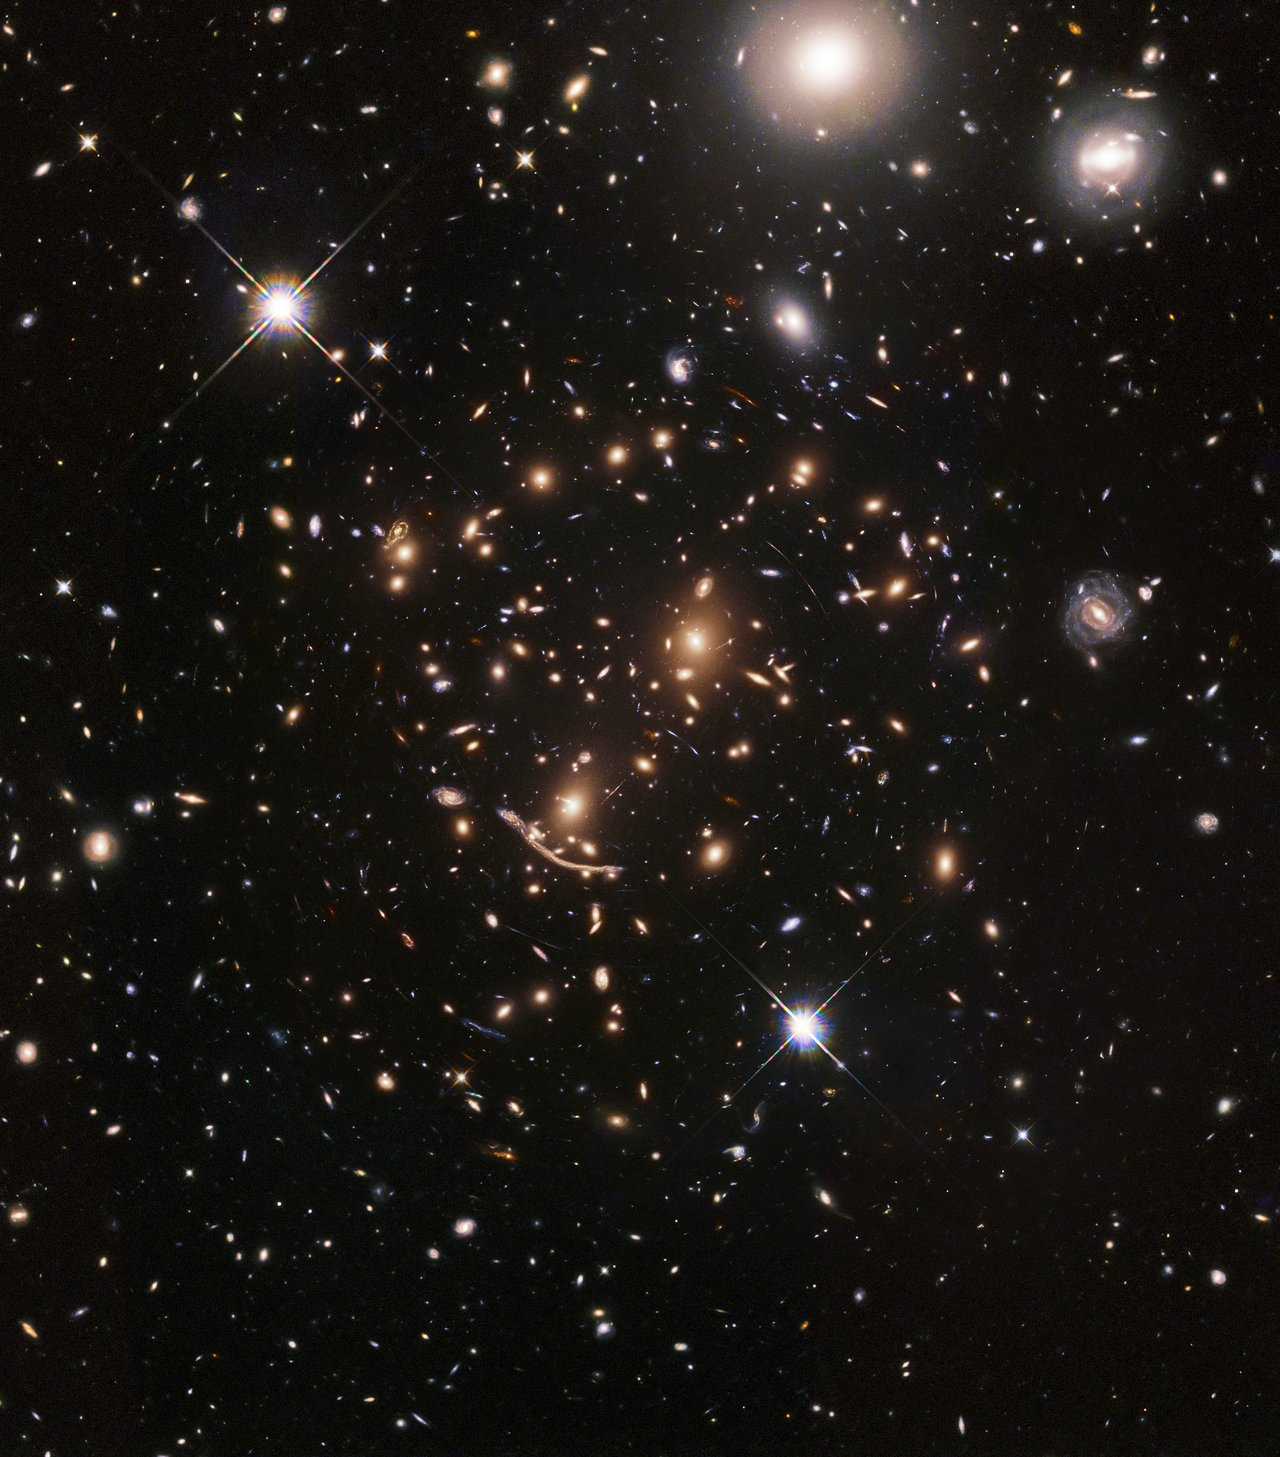
\includegraphics[width=0.6\textwidth]{../figures/universe.jpeg}}
		\end{figure}
	
\end{frame}

\begin{frame}
	\frametitle{What does it mean to understand the universe?}
	
	\begin{figure}[ht]
		\centerline{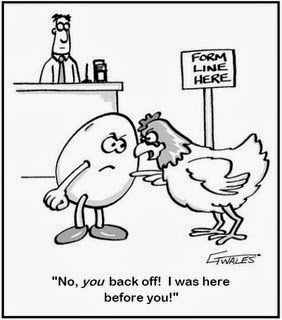
\includegraphics[width=0.5\textwidth]{../figures/chicken_egg.jpeg}}
	\end{figure}
	
\end{frame}

\begin{frame}
	\frametitle{Why do we need data and statistics?}
	
	\Large
	Question: can't we just use data we collect?
	
\end{frame}

\begin{frame}
	\frametitle{Nate Silver}
	
	\begin{figure}[ht]
		\centerline{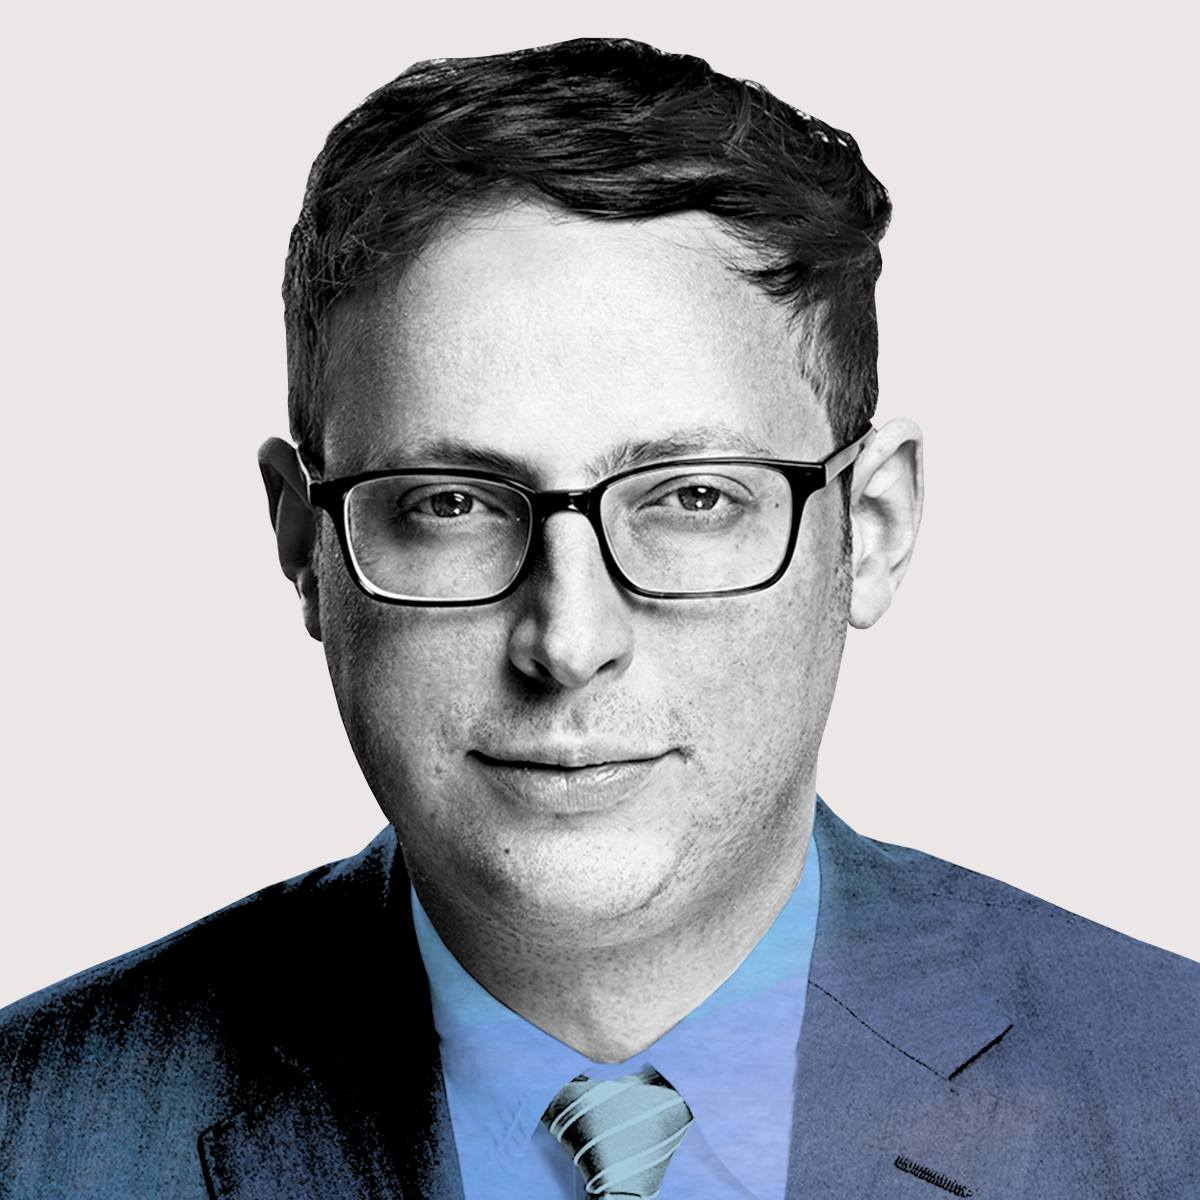
\includegraphics[width=0.5\textwidth]{../figures/natesilver.jpeg}}
	\end{figure}
	
	``The numbers have no way of speaking for themselves. We speak for them. We imbue them with meaning.''
	
\end{frame}

\begin{frame}
	\frametitle{But why do we need statistics?}
	
	\begin{itemize}
		\item The universe is complex
		\item Its mechanisms are not directly observable
		\item Our data contain information both about the mechanisms and other nuisance factors
	\end{itemize}
	
	$\implies$ we need to make assumptions that separate signal from noise
	
\end{frame}

\begin{frame}
	\frametitle{How statistics separates signal from noise?}
	
	\begin{equation}
	\text{observations} = \text{signal} + \text{noise}
	\end{equation}
	
	\begin{itemize}
		\item Signal contains our interesting scientific mechanism
		\item Noise contains a bunch of things not of interest
	\end{itemize}
	
	Since we do not know or observe the exact noise processes, in statistics, it is assumed that the noise is represented as being \textit{random}.
	
	\vspace{0.5cm}
	
	But random does not mean unstructured. In statistics, making assumptions about the nature of the random process allows us to bound its influence on the observed data.
	
\end{frame}

\begin{frame}
	\frametitle{Example 1: flipping a coin}
	
	Suppose we flip a coin twice. We could obtain:
	
	\begin{itemize}
		\item Two tails
		\item One head; one tail
		\item Two heads
	\end{itemize}
	
	Why can we get different outcomes each time the coin is flipped?
	
\end{frame}

\begin{frame}
	\frametitle{Different initial conditions}
	
	Precessional frequency: $\omega_N$; Magnitude of upward velocity, $u$.\footnote{\tiny From Probability, geometry, and dynamics in the toss of a thick coin, Yong and Mahadevan (2011)}
	
	\begin{figure}[ht]
		\centerline{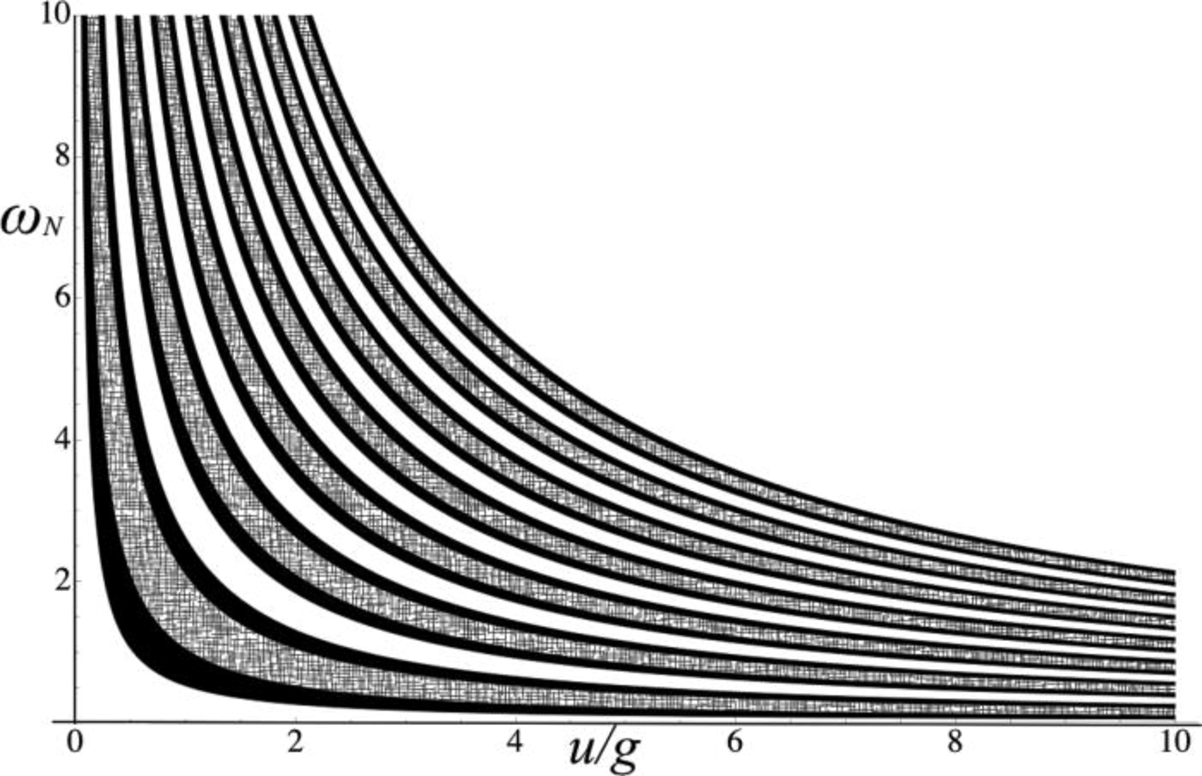
\includegraphics[width=0.6\textwidth]{../figures/coin_toss.pdf}}
	\end{figure}
	
	White indicates heads; hatched indicates lands on sides; black indicates tails.
	
\end{frame}

\begin{frame}
	\frametitle{Coin flip dynamics: physics approach}
	
	Solve complex equations of motion (making assumptions about flipping process). One part of the system:
	
	\begin{equation}
	\frac{d\boldsymbol{N}}{dt} = \Omega \times \boldsymbol{N}
	\end{equation}
	
	This system determines outcome given a set of initial conditions: precessional frequency and magnitude of upward velocity.
	
	\vspace{0.5cm}
	But we still don't know how different people throw a coin, so we'd need to measure this and likely represent this using randomness!
	
\end{frame}

\begin{frame}
	\frametitle{Coin flip dynamics: statistical approach}
	
	Assume outcome of a coin flip is a random variable with a probability of landing heads up (binomial distribution\footnote{If we forget the landing on side situation.}). Implicitly:
	
	\begin{figure}[ht]
		\centerline{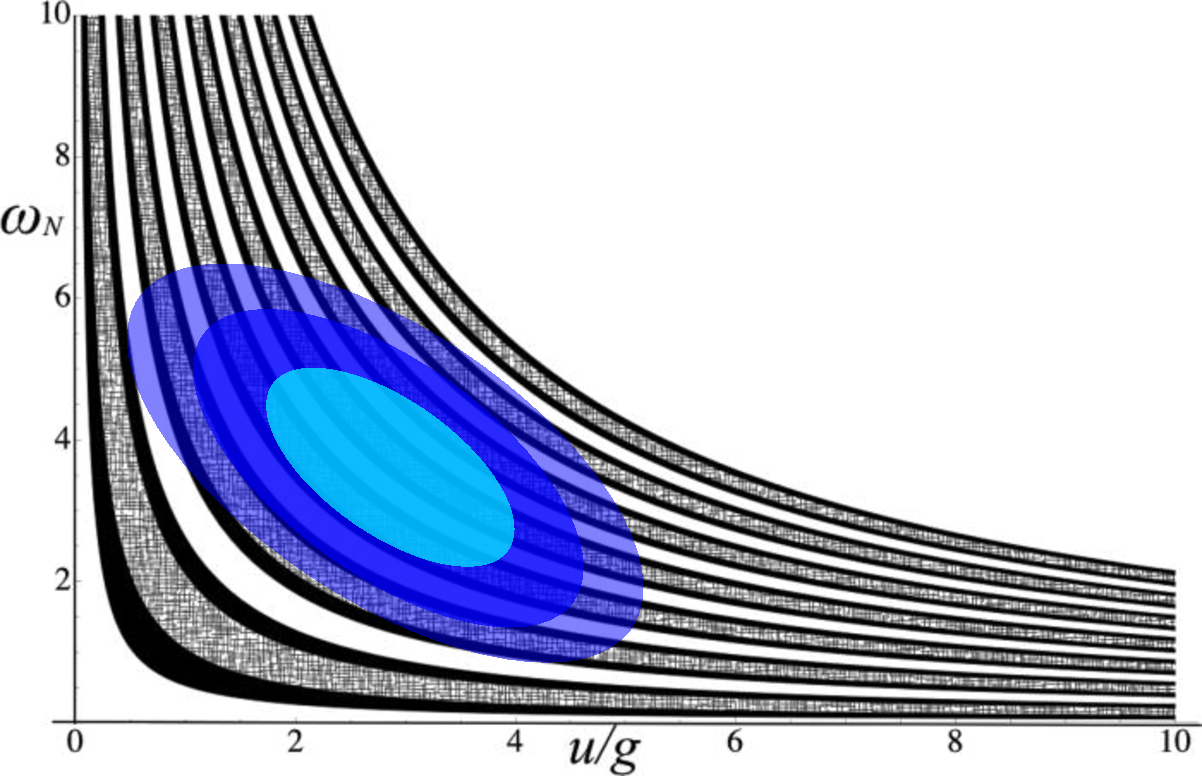
\includegraphics[width=0.6\textwidth]{../figures/coin_toss_density.pdf}}
	\end{figure}
	
\end{frame}

\begin{frame}
	\frametitle{Example 2: determining COVID-19 seropositivity}
	Imagine we want to determine the proportion of the UK population who have COVID-19 antibodies. To do this, we find 10 individuals and test their blood.
	
	\begin{figure}[ht]
		\centerline{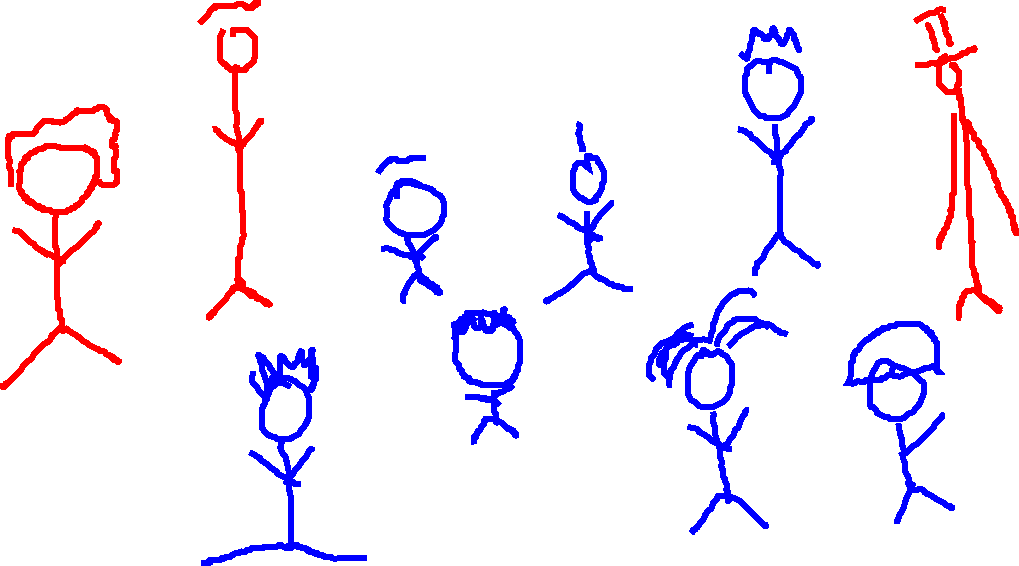
\includegraphics[width=0.6\textwidth]{../figures/covid_stick.pdf}}
	\end{figure}
	
	Does this mean $3/10=30\%$ of the UK population have these antibodies?
	
\end{frame}

\begin{frame}
	\frametitle{The sampling process yields variation in outputs}
	No.
	
	\begin{figure}[ht]
		\centerline{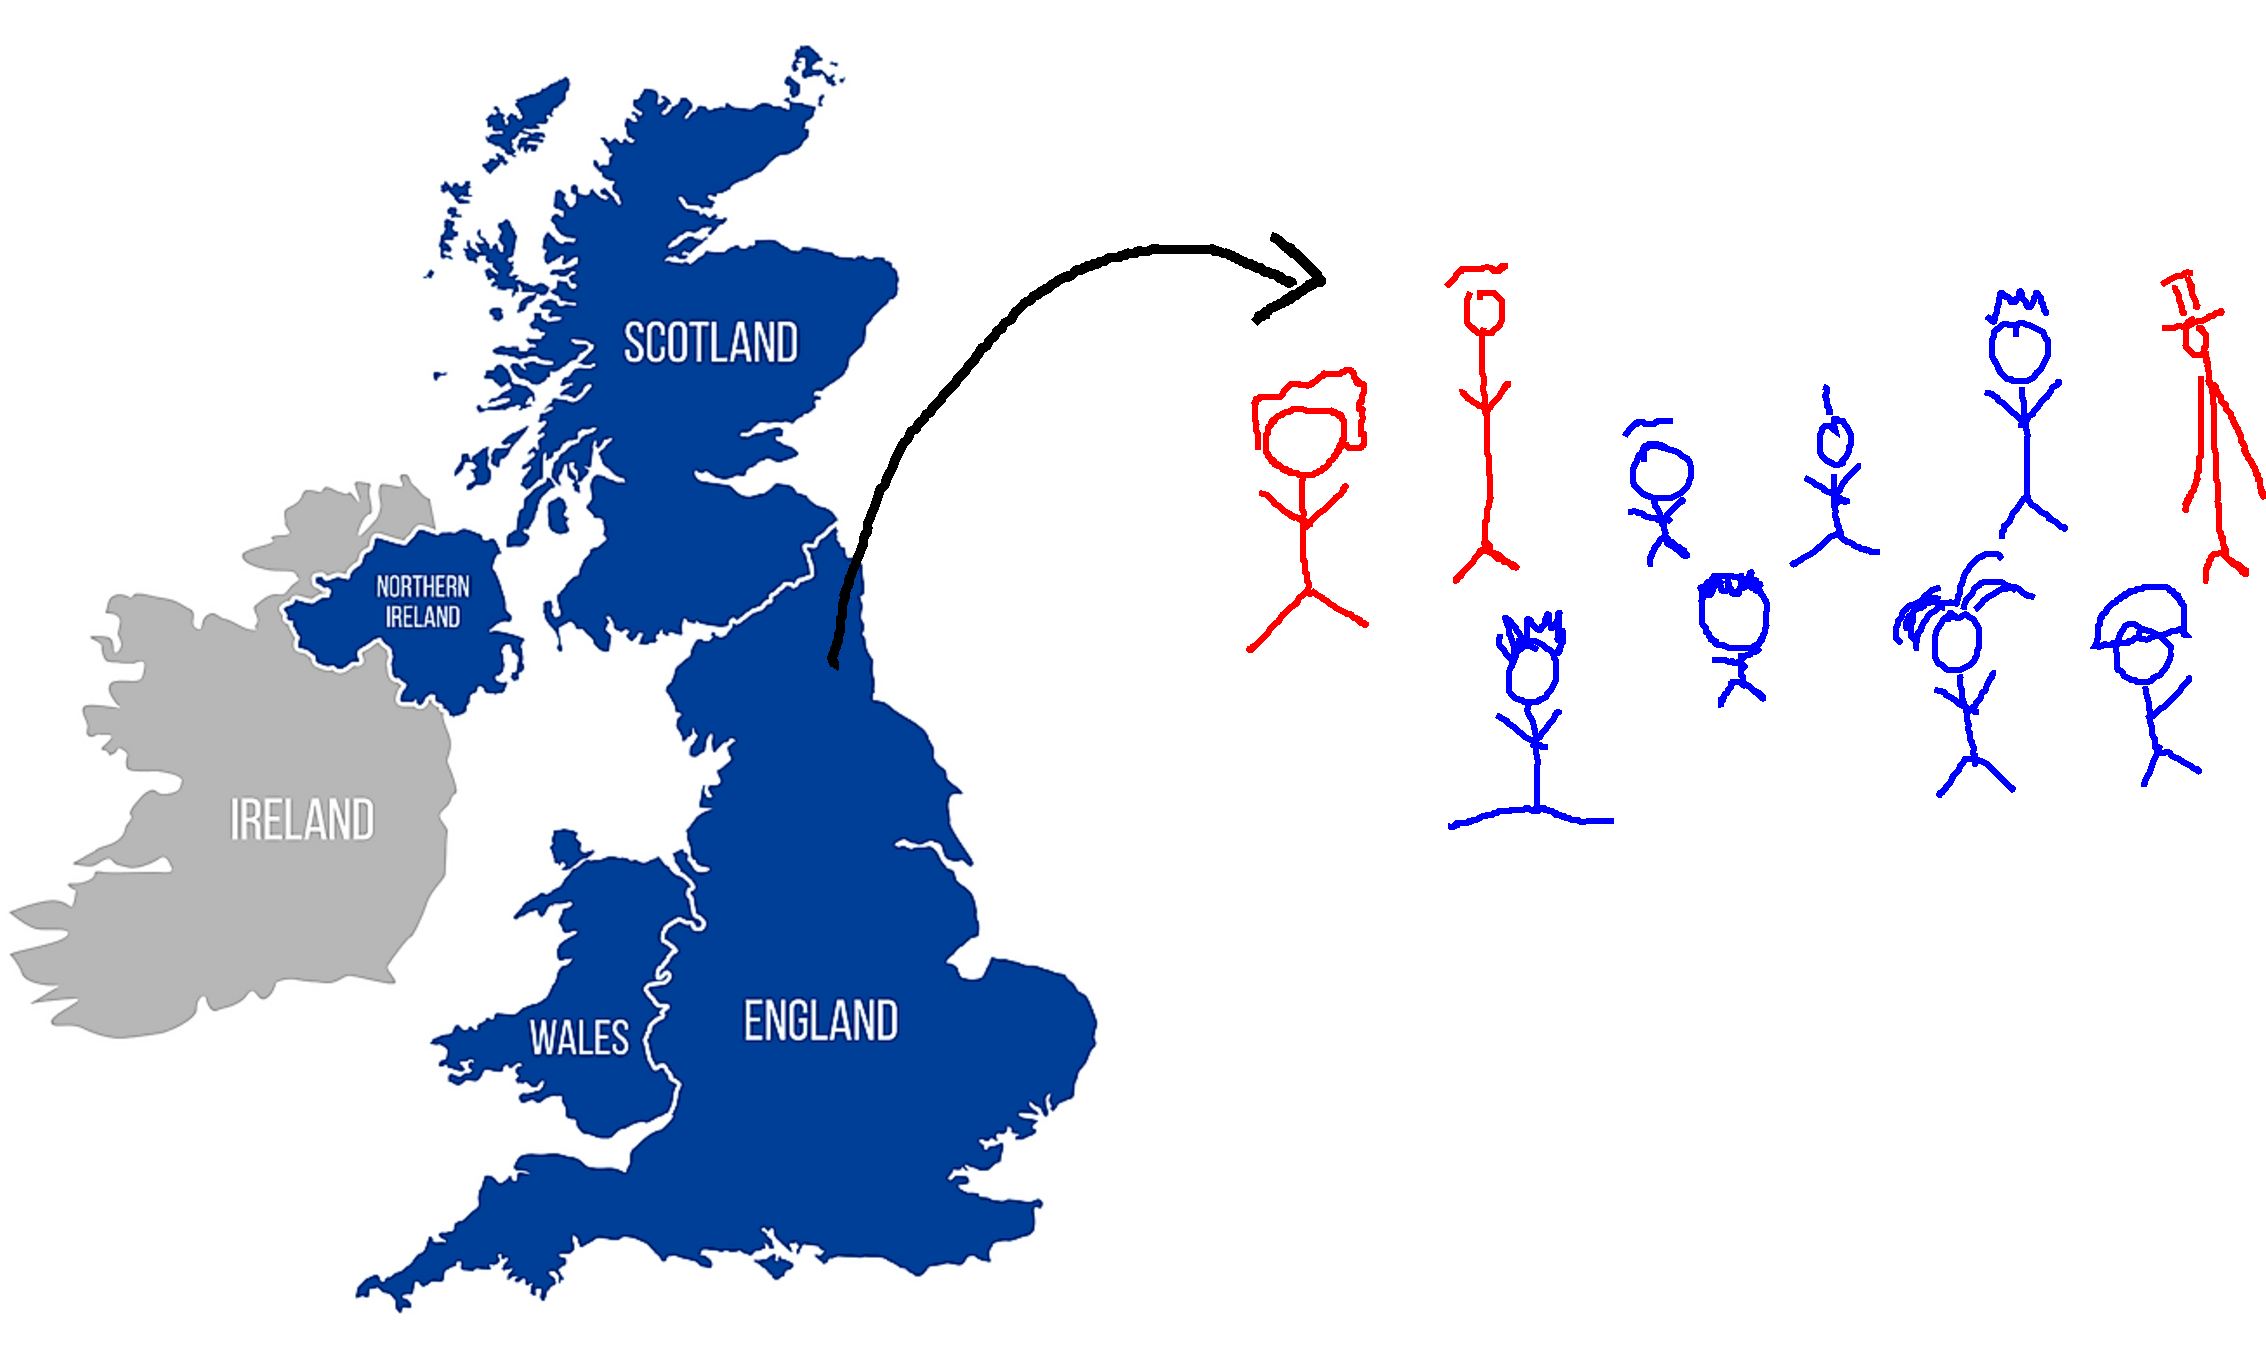
\includegraphics[width=1\textwidth]{../figures/uk-population.pdf}}
	\end{figure}
	
\end{frame}

\section{Can statistics help to determine causation?}
\frame{\tableofcontents[currentsection]}


\begin{frame}
	\frametitle{Correlation and causation}
	
	\begin{figure}[ht]
		\centerline{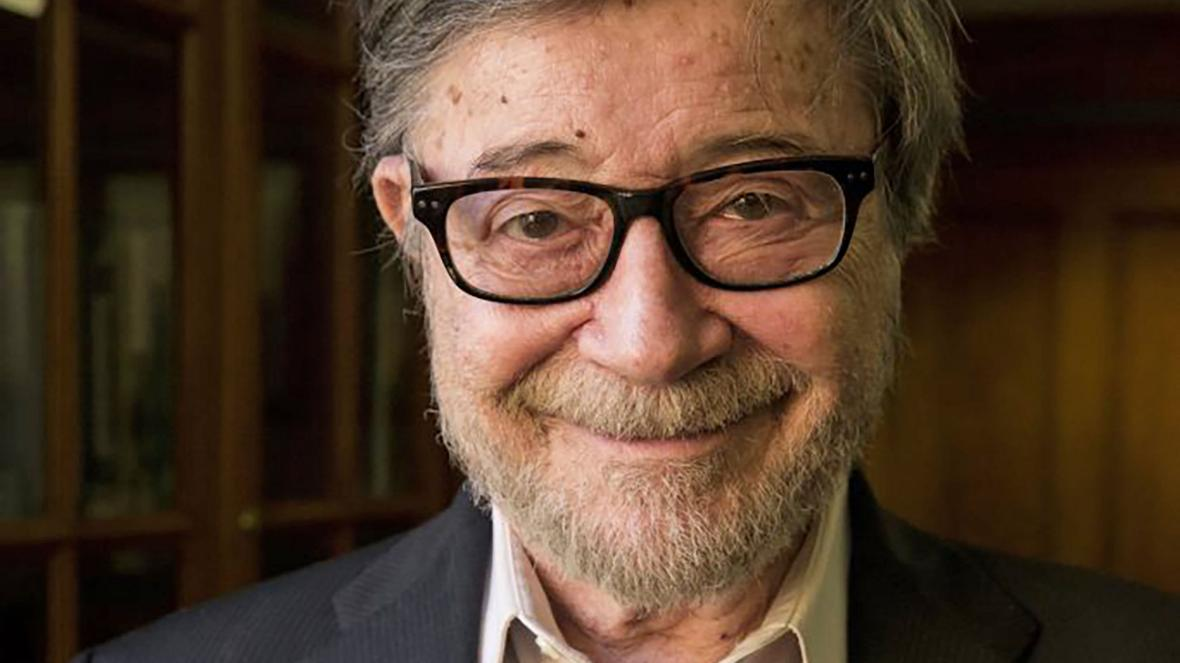
\includegraphics[width=0.5\textwidth]{../figures/judea_pearl.jpeg}}
	\end{figure}
	
	``"Correlation is not causation". With good reason! The rooster's crow is highly correlated with the sunrise; yet it does not cause the sunrise. Unfortunately, statistics has fetishized this commonsense observation. It tells us that correlation is not causation, but it does not tell us what causation is.''
	
\end{frame}

\begin{frame}
	\frametitle{Smoking and lung cancer: how did we get here?}
	
	\begin{columns}
		\begin{column}{0.48\textwidth}
			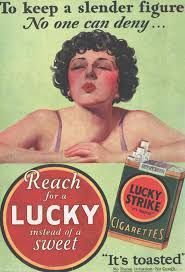
\includegraphics[width=0.9\textwidth]{../figures/cigarette_early1.jpeg}
		\end{column}
		\begin{column}{0.48\textwidth}
			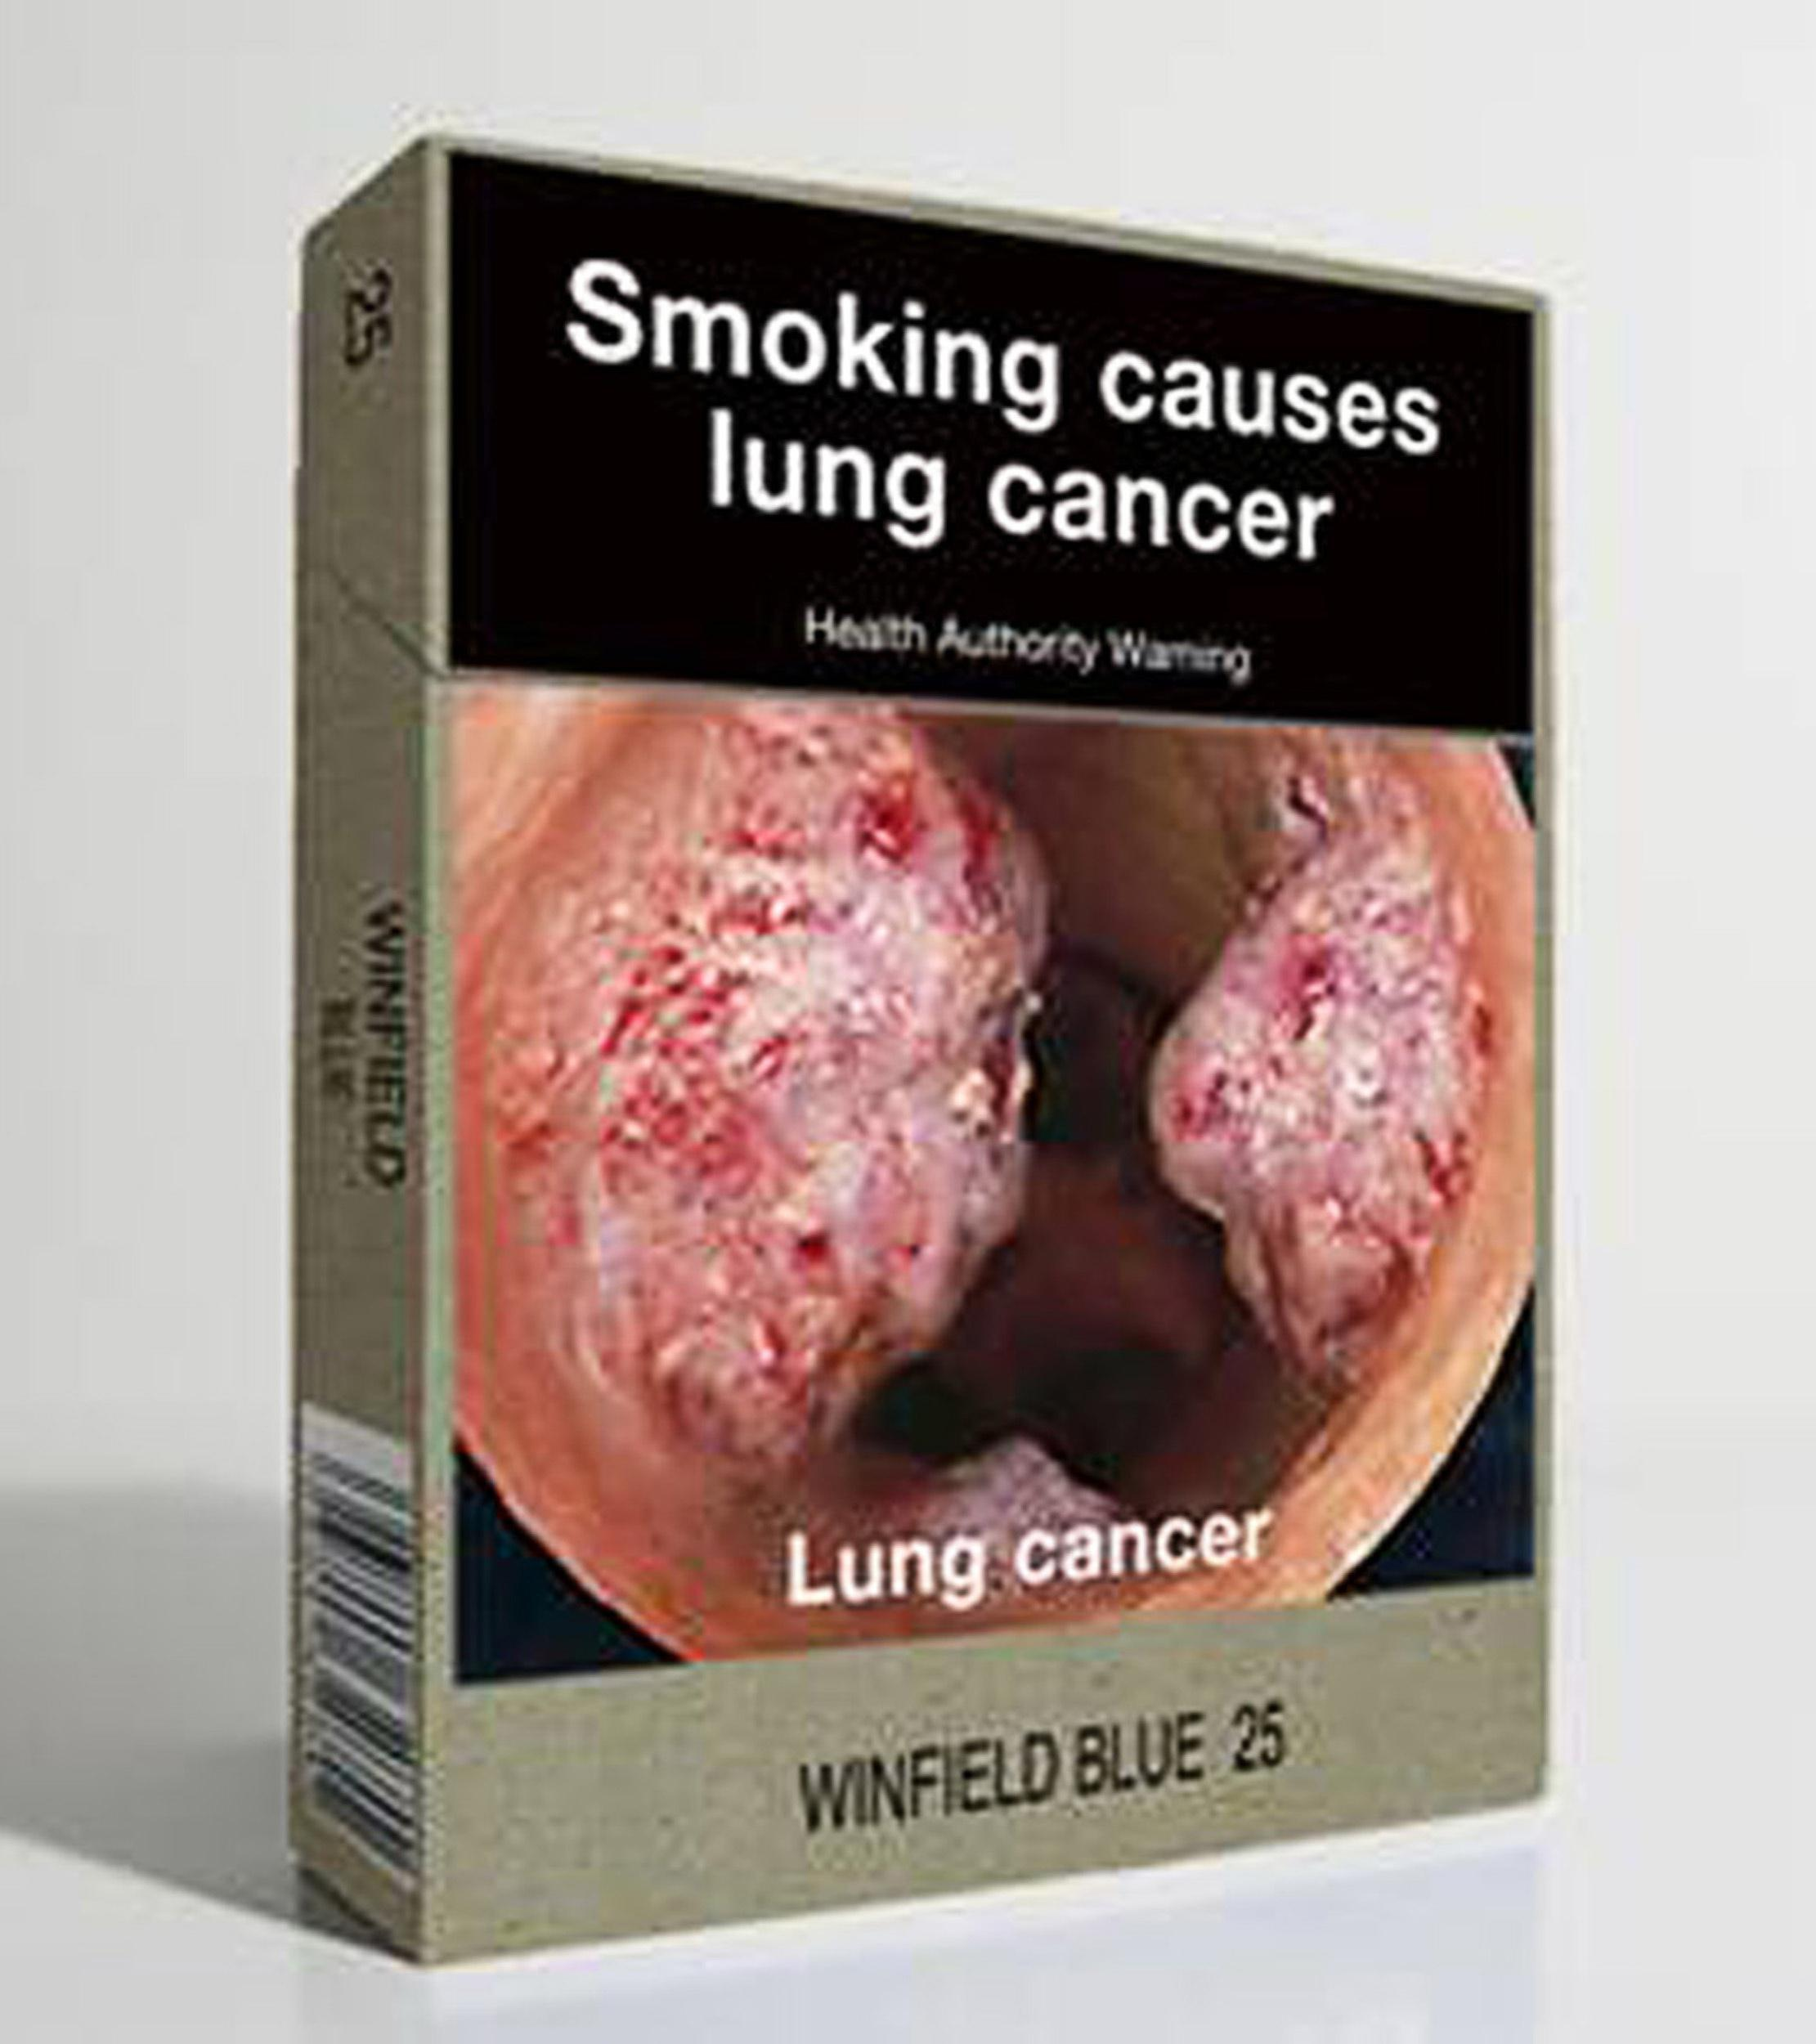
\includegraphics[width=0.9\textwidth]{../figures/cigarette_late.jpeg}
		\end{column}
	\end{columns}
	
\end{frame}

\begin{frame}
	\frametitle{Experiments: easier but immoral}
	
	\begin{figure}[ht]
		\centerline{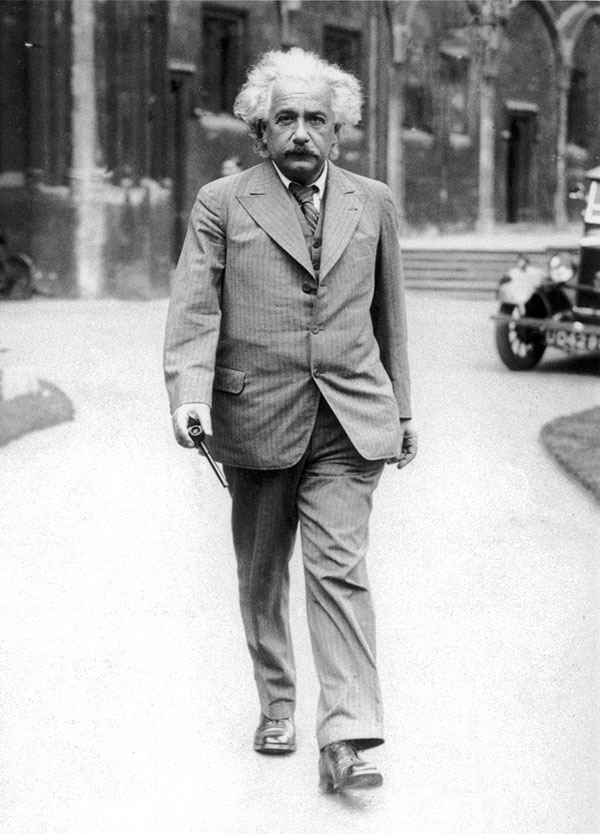
\includegraphics[width=0.3\textwidth]{../figures/einstein_oxford.jpeg}}
	\end{figure}
	
	``Development of Western science is based on two great achievements: the invention of the formal logical system (in Euclidean geometry) by the Greek philosophers, and the discovery of the possibility to find out causal relationships by systematic experiment (during the Renaissance).''
	
\end{frame}

\begin{frame}
	\frametitle{Occurrence of lung cancer: early on}
	
	\begin{quotation}
		Lung cancer was once a very rare disease, so rare that doctors took special notice when confronted with a case, thinking it a once-in-a-lifetime oddity.
	\end{quotation}
	
	\begin{quotation}
		Lung cancer was not even recognised medically until the 18th century, and as recently as 1900 only about 140 cases were known in the published medical literature.
	\end{quotation}
	
	\footnotesize Both taken from ``The history of the discovery of the cigarette-lung cancer link: evidentiary traditions, corporate denial, global toll'', Proctor, \textit{Tobacco Control} 2012.
	
\end{frame}

\begin{frame}
	\frametitle{Correlation: early-mid twentieth century}
	
	\begin{figure}[ht]
		\centerline{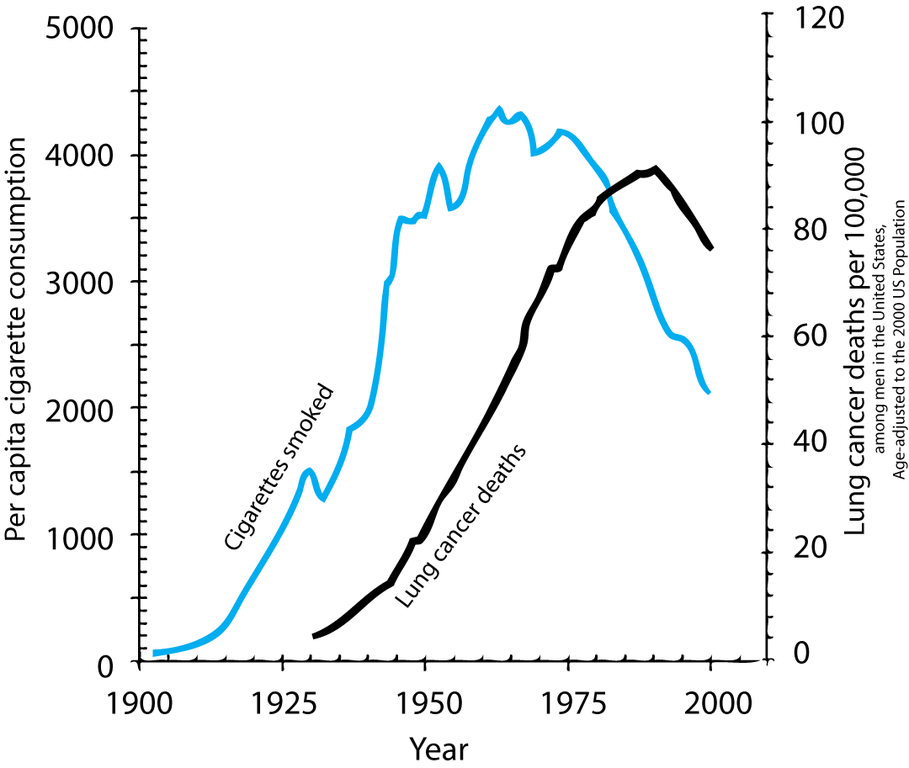
\includegraphics[width=0.8\textwidth]{../figures/smoking_cancer.png}}
	\end{figure}
	
\end{frame}

\begin{frame}
	\frametitle{Case-control: Doll and Hill, 1950}
	
	\begin{figure}[ht]
		\centerline{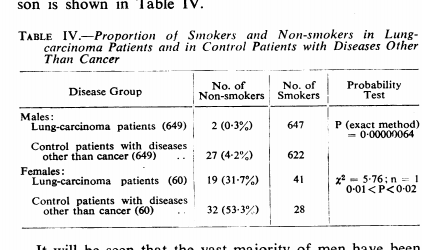
\includegraphics[width=0.8\textwidth]{../figures/doll_hill_table}}
	\end{figure}
	\footnotesize ``Smoking and carcinoma of the lung'', Doll and Hill, \textit{BMJ} 1950.
\end{frame}

\begin{frame}
	\frametitle{Prospective cohort study: Doll and Hill, 1954}
	
	Study of over 40,000 doctors.
	
	\begin{figure}[ht]
		\centerline{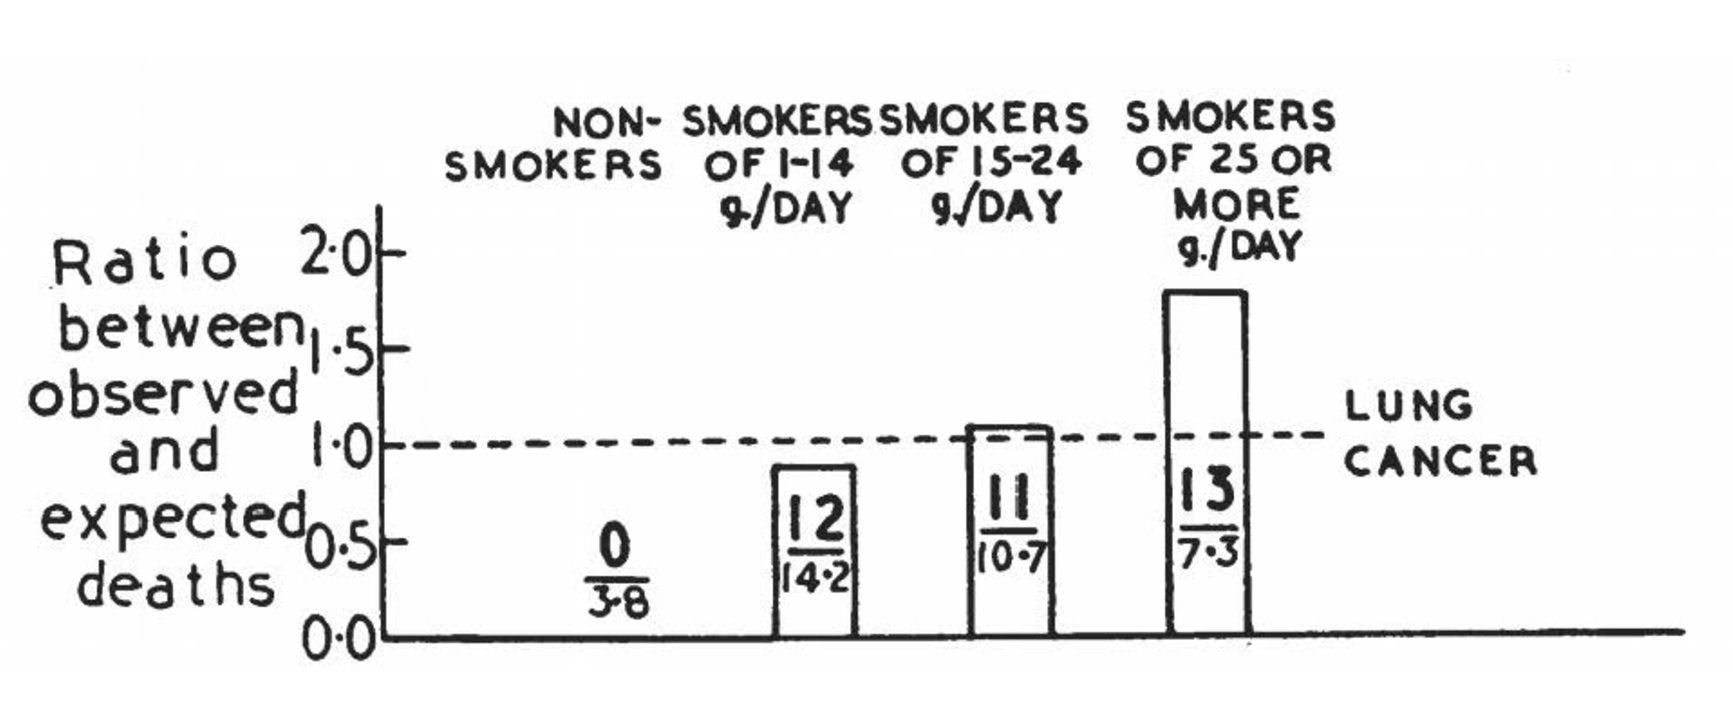
\includegraphics[width=0.8\textwidth]{../figures/doll_hill_1954.pdf}}
	\end{figure}
	
	\footnotesize ``The mortality of doctors in relation to their smoking habits'', Doll and Hill, \textit{BMJ} 1950.
	
\end{frame}

\begin{frame}
	\frametitle{Other sources of causal evidence}
	
	Animal studies:
	\begin{itemize}
		\item 1931: Roffo showed that smoke condensed from distillation of tobacco caused tumours when smeared on skins of rabbits
		\item 1953 Wynder, Graham and Croninger showed tumours could be generated by painting cigarette smoke tar onto backs of shaved mice
	\end{itemize}
	
	Cellular pathology:
	\begin{itemize}
		\item 1956: Hilding demonstrated that smokers experienced ciliastasis and that the cilia were being deadened at parts of lung wear cancers likely to develop
	\end{itemize}
	
\end{frame}

\begin{frame}
	\frametitle{Other sources of causal evidence}
	
	Chemicals known to cause cancer in cigarette smoke:
	\begin{itemize}
		\item 1939: Roffo found polycyclic aromatic hydrocarbons in cigarette smoke, which had already been identified as carcinogenic components of coal tar
		\item 1952: Brown and Williamson identified benzpyrene in cigarette smoke
		\item End of 1950s: cigarette manufacturers had characterised several dozen carcinogens in cigarette smoke
	\end{itemize}
	
\end{frame}

\begin{frame}
	\frametitle{Path to causal link between smoking and lung cancer}
	
	\begin{itemize}
		\item Unethical to perform experiments on humans
		\item Statistical analysis of observational data played a key role
		\item Confluence of diverse forms of evidence
	\end{itemize}
	
	1954: a number of national health bodies advised that stopping smoking could prevent cancer
	
\end{frame}

\begin{frame}
	\frametitle{How to conclude causality from observational data}
	In 1965, Austin Hill set out a list of criteria to be considered before concluding that a causal link exists between an exposure and an outcome.
	Direct evidence:
	\begin{itemize}
		\item Effect size so large that can't be explained by confounders
		\item Appropriate temporal and/or spatial proximity
		\item Dose responsiveness and reversibility
	\end{itemize}
	
	Mechanistic evidence:
	\begin{itemize}
		\item There exists a plausible mechanism of action: biological, chemical, mechanical and so on
	\end{itemize}
	
	Parallel evidence:
	\begin{itemize}
		\item Fits with what is known already
		\item Effect found when study replicated
		\item Effect found in similar, but not identical studies
	\end{itemize}
	
\end{frame}


\section{Estimating interesting quantities using regression}
\frame{\tableofcontents[currentsection]}

\begin{frame}
	\frametitle{Example: Galton's 1885 study of 205 families (898 children)}
	
	Question: how inheritable is height from parent to child?
	
		\begin{figure}[ht]
			\centerline{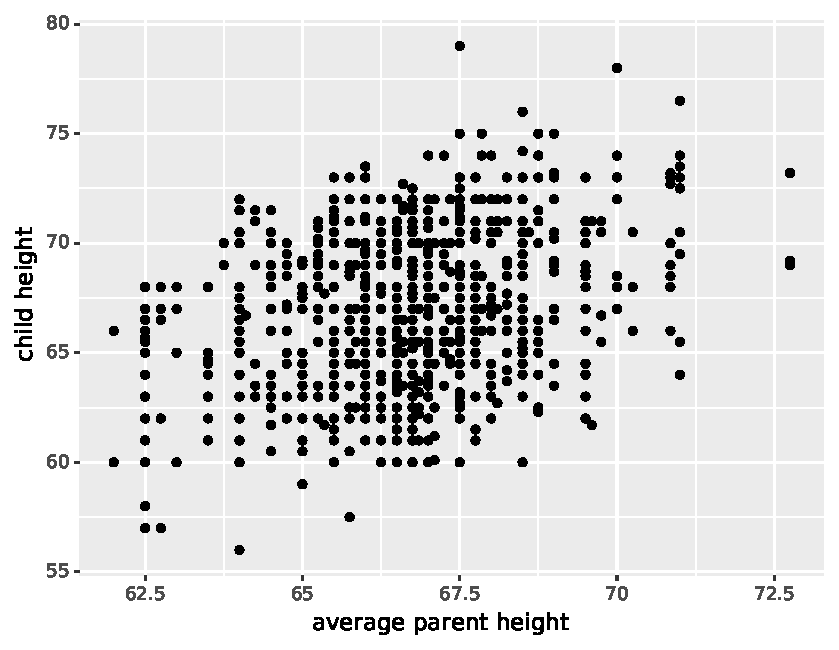
\includegraphics[width=0.9\textwidth]{../figures/galton_raw.pdf}}
		\end{figure}
	
\end{frame}

\begin{frame}
	\frametitle{Potential model}
	
	Suppose child height linearly related to parent height:
	
	\begin{equation}
	\text{child}_i = a + b * \text{parent}_i.
	\end{equation}
	
	Here, $b$ represents the effect of interest:
	
	\begin{itemize}
		\item $b=1 \implies$ a 1 inch increase in average parent height is associated with a 1 inch increase in child height.
		\item $b=0 \implies$ no relationship.
	\end{itemize}
	
	This isn't a causal model, so doesn't directly answer our heritability question. But it is still useful.
	
	\vspace{0.5cm}
	
	Important: this is a model: a simplified version of reality. It embodies a number of assumptions.
	
\end{frame}

\begin{frame}
	\frametitle{Example models}
	
	\begin{figure}[ht]
		\centerline{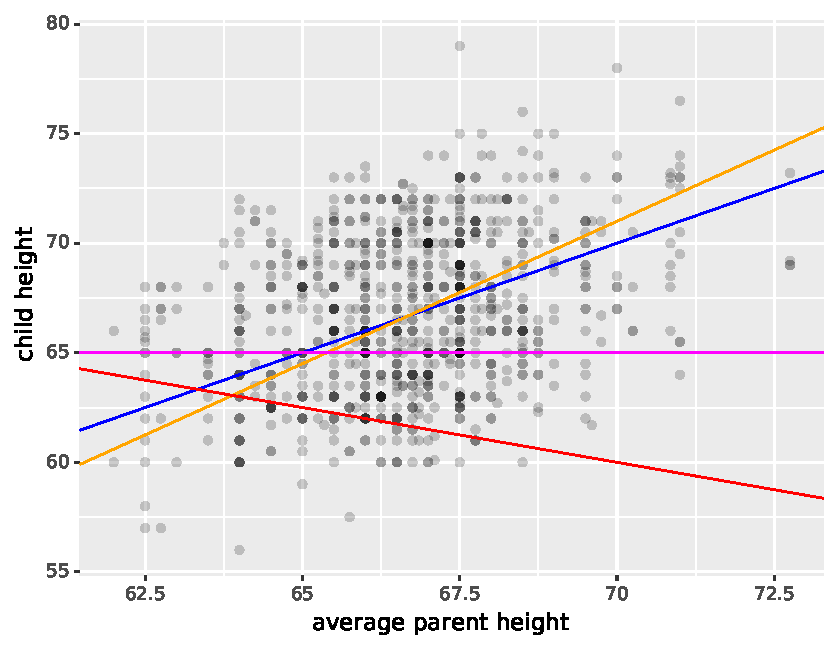
\includegraphics[width=0.9\textwidth]{../figures/galton_example_lines.pdf}}
	\end{figure}
	
\end{frame}

\begin{frame}
	\frametitle{What's the problem with this model?}
	
	It doesn't provide a mechanism to exactly hit data.
	
	\begin{figure}[ht]
		\centerline{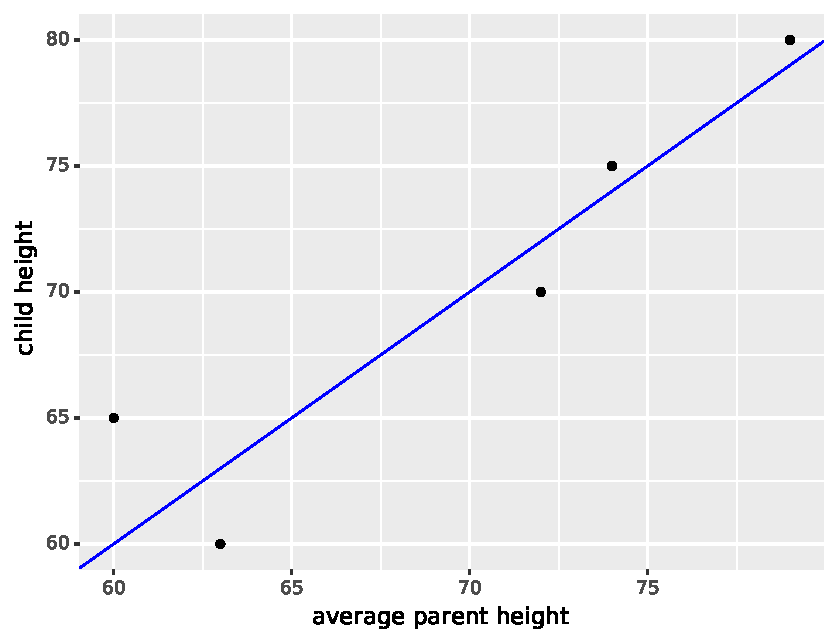
\includegraphics[width=0.9\textwidth]{../figures/galton_model_without_residuals.pdf}}
	\end{figure}
	
\end{frame}

\begin{frame}
	\frametitle{How to modify the model}
	
	\begin{equation}
	\text{child}_i = a + b * \text{parent}_i + \epsilon_i.
	\end{equation}
	
	where $\epsilon_i$ is a random error term representing the myriad of other factors not captured by the other parts of the model.
	
\end{frame}

\begin{frame}
	\frametitle{What does this model look like?}
	
	\begin{figure}[ht]
		\centerline{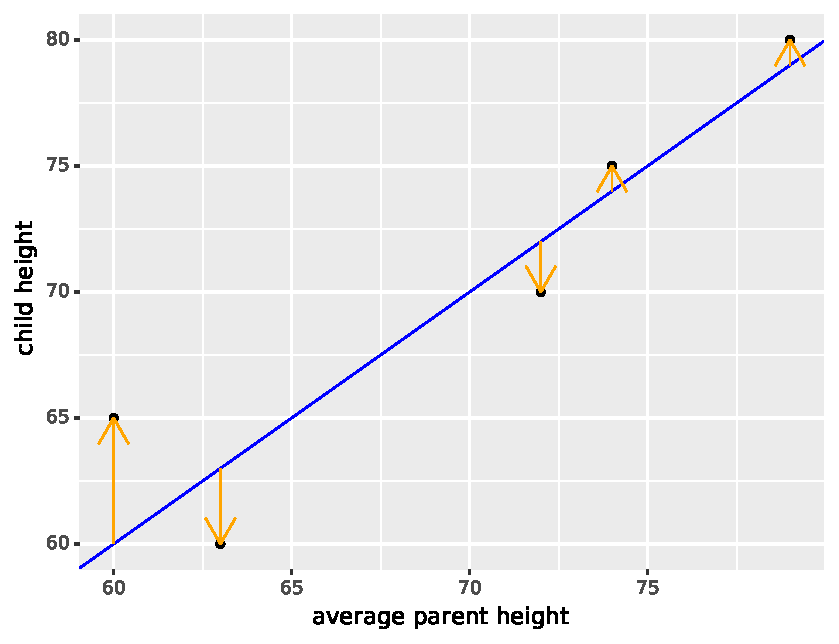
\includegraphics[width=0.9\textwidth]{../figures/galton_model_with_residuals.pdf}}
	\end{figure}
	
\end{frame}

\begin{frame}
	\frametitle{How to estimate the model's parameters from data?}
	
	Want the non-random parts of the model to explain most variation.
	
	\vspace{0.5cm}
	
	So, choose $(a,b)$ so that they minimise some measure of distance between points and line. For example, sum of squared errors:
	
	\begin{equation}
	d = \sum_{i=1}^{N} (\text{child}_i - a - b * \text{parent}_i)^2
	\end{equation}
	
\end{frame}

\begin{frame}
	\frametitle{Sum of squared errors fit}
	
	\begin{figure}[ht]
		\centerline{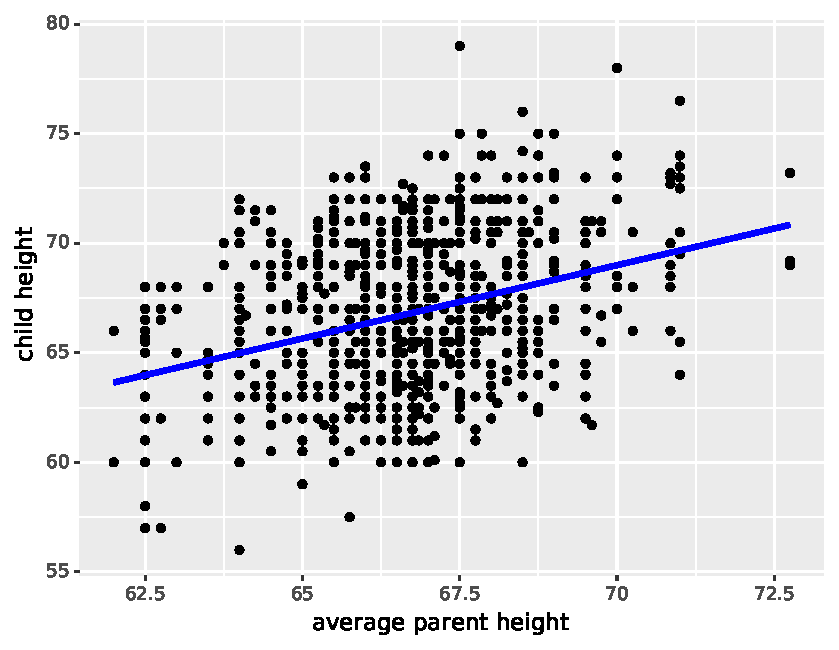
\includegraphics[width=0.9\textwidth]{../figures/galton_fit_sse.pdf}}
	\end{figure}
	
\end{frame}

\begin{frame}
	\frametitle{Other distance measures}
	
	Could have chosen the sum of absolute distances instead:
	
	\begin{equation}
	d = \sum_{i=1}^{N} |\text{child}_i - a - b * \text{parent}_i|
	\end{equation}
	
	Or of fourth power:
	
	\begin{equation}
	d = \sum_{i=1}^{N} (\text{child}_i - a - b * \text{parent}_i)^4
	\end{equation}
		
	Question: how would these choices affect the fit?
	
\end{frame}

\begin{frame}
	\frametitle{Various fits}
	
		\begin{figure}[ht]
			\centerline{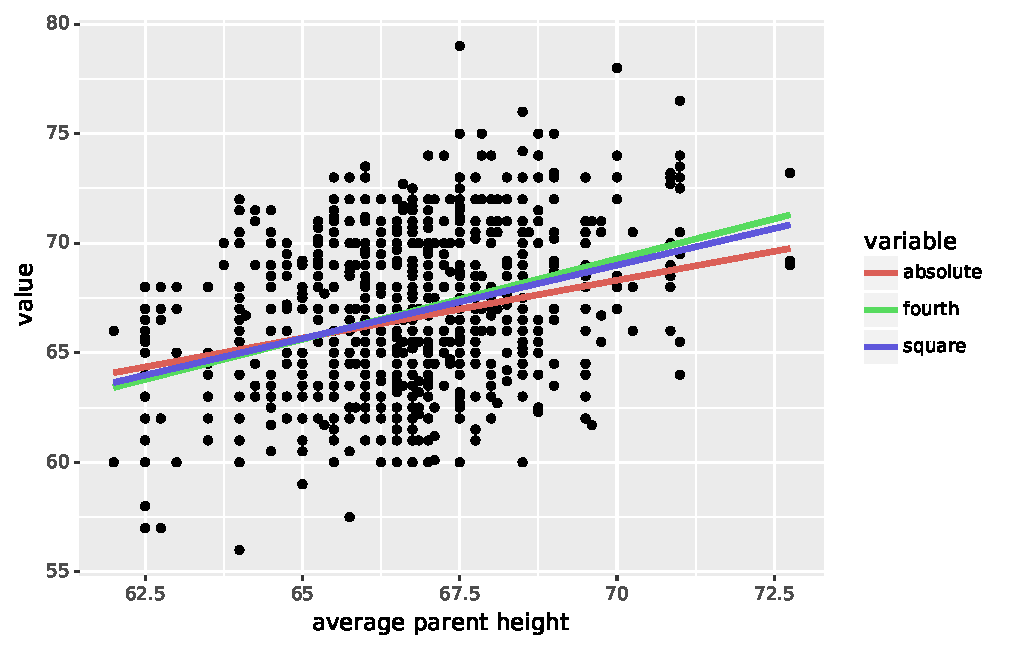
\includegraphics[width=0.9\textwidth]{../figures/galton_fits_all.pdf}}
		\end{figure}
		
		Conclude: subjective choice of 'distance' affects our estimates.
	
\end{frame}

\begin{frame}
	\frametitle{A more principled probability-based approach}
	
	Assume:
	
	\begin{equation}
	\text{child}_i = a + b * \text{parent}_i + \epsilon_i,
	\end{equation}
	
	where $\epsilon_i \sim \text{normal}(0, \sigma)$.
	
\end{frame}

\begin{frame}
	\frametitle{What does this model look like? Draw}
	
	\begin{figure}[ht]
		\centerline{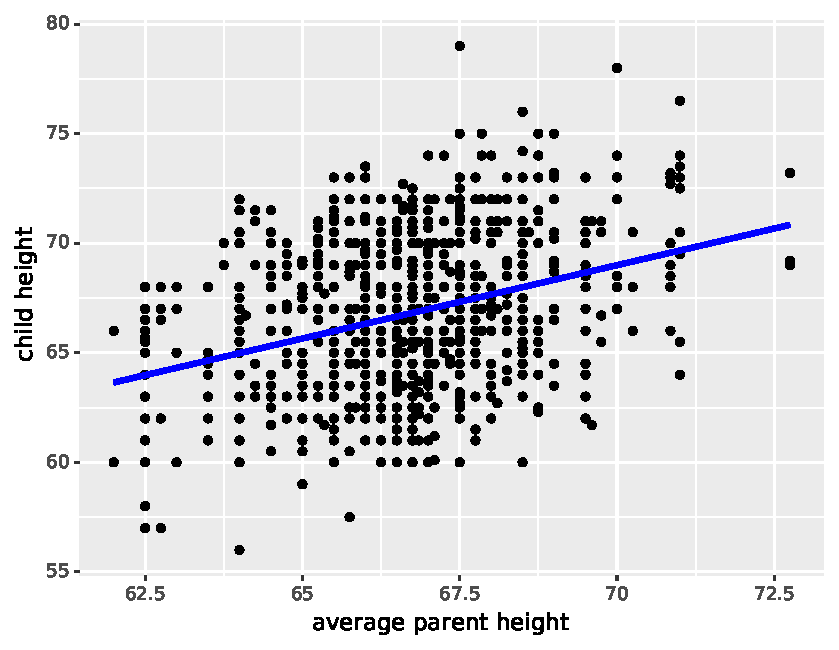
\includegraphics[width=0.9\textwidth]{../figures/galton_fit_sse.pdf}}
	\end{figure}
	
\end{frame}

\begin{frame}
	\frametitle{But isn't a normal distribution also arbitrary?}
	
	No! Why? The central limit theorem. 
	
	\vspace{0.5cm}
	
	Suppose we flip a fair coin once. What does its probability distribution look like?
	
\end{frame}

\begin{frame}
	\frametitle{One coin flip}
	
	\begin{figure}[ht]
		\centerline{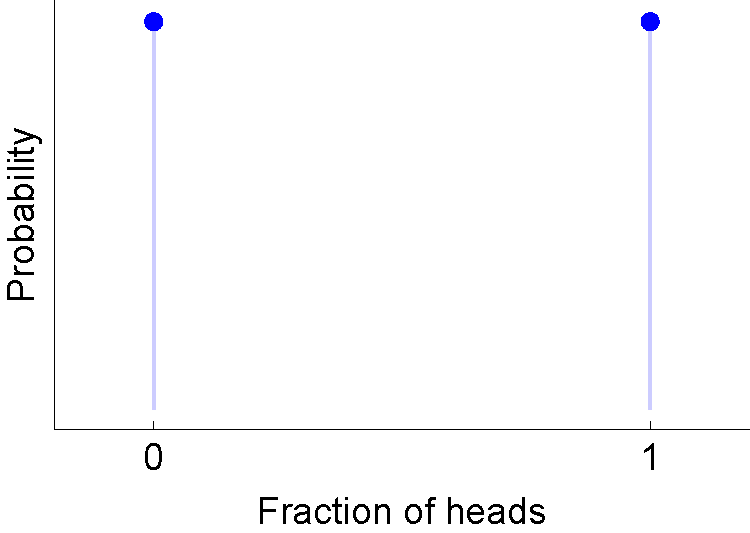
\includegraphics[width=0.9\textwidth]{../figures/binomial_1.pdf}}
	\end{figure}
	
\end{frame}

\begin{frame}
	\frametitle{Two flips}
	I now flip the coin 2 times.
	
	\vspace{0.5cm}
	
	Question: What does the distribution look like now?
	
\end{frame}

\begin{frame}
	\frametitle{Two flips flips}
	
	\begin{figure}[ht]
		\centerline{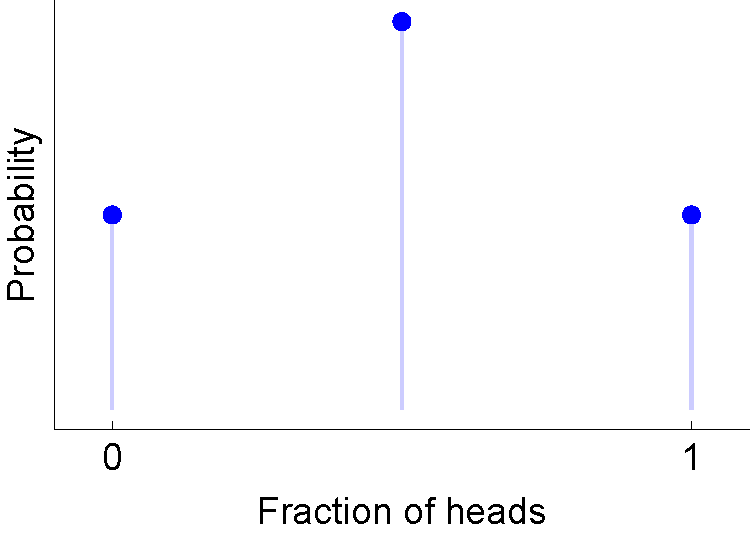
\includegraphics[width=0.9\textwidth]{../figures/binomial_2.pdf}}
	\end{figure}
	
\end{frame}

\begin{frame}
	\frametitle{What about five flips?}
	
	
\end{frame}

\begin{frame}
	\frametitle{What about five flips?}
	
	\begin{figure}[ht]
		\centerline{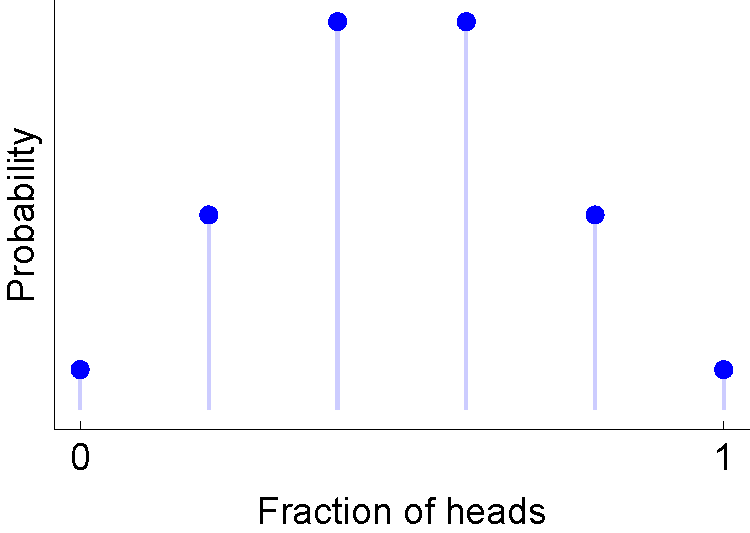
\includegraphics[width=0.9\textwidth]{../figures/binomial_5.pdf}}
	\end{figure}
	
\end{frame}

\begin{frame}
	\frametitle{What about 30 flips?}
	
	\begin{figure}[ht]
		\centerline{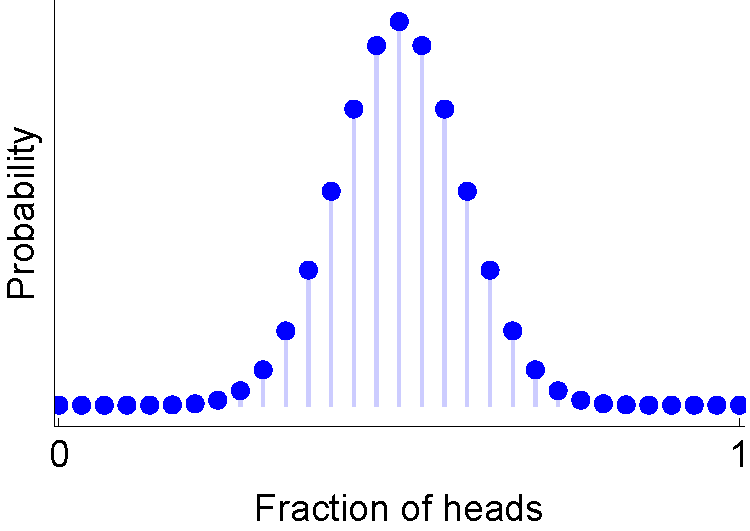
\includegraphics[width=0.9\textwidth]{../figures/binomial_30.pdf}}
	\end{figure}
	
\end{frame}

\begin{frame}
	\frametitle{What's going on?}
	The Central Limit Theorem (CLT) says that under general conditions:
	
	\vspace{0.5cm}
	
	``The distribution of the average of a large number of weakly dependent random variables is approximately normal.''
	
	\vspace{0.5cm}
	
	In the coin flipping case, we effectively calculated the average number of independent coin flips landing heads up $\implies$ CLT applies.
	
\end{frame}

\begin{frame}
	\frametitle{Back to our regression example}

	\begin{equation}
	\text{child}_i = a + b * \text{parent}_i + \epsilon_i,
	\end{equation}
	
	where $\epsilon_i \sim \text{normal}(0, \sigma)$.
	
	\vspace{0.5cm}
	
	Large number of weakly dependent factors -- genetic, environmental and so-forth -- likely influence a person's height.
	
	$\implies$
	
	CLT applies, so normal distribution may be appropriate.
	
\end{frame}

\begin{frame}
	\frametitle{Likelihood based inference}
	
	\begin{equation}
	\text{child}_i = a + b * \text{parent}_i + \epsilon_i,
	\end{equation}
	
	and
	
	\begin{equation}
	\epsilon_i \sim \text{normal}(0, \sigma),
	\end{equation}
	
	means that:
	
	\begin{equation}
	\text{child}_i - a - b * \text{parent}_i\sim \text{normal}(0, \sigma).
	\end{equation}
	
	This provides us with a way of writing down the overall probability (density) of observations.
	
\end{frame}

\begin{frame}
	\frametitle{Likelihood}
	
	Due to independence of observations:
	
	\begin{align}
	\mathcal{L} = &\mathbb{P}(\epsilon_1) \times \mathbb{P}(\epsilon_2) \times ... \times  \mathbb{P}(\epsilon_n)\\
	= &\text{normal}(\text{child}_1 - a - b * \text{parent}_1|0, \sigma) \times\\
	&\text{normal}(\text{child}_2 - a - b * \text{parent}_2|0, \sigma)\\
	&...\\
	&\text{normal}(\text{child}_n - a - b * \text{parent}_n|0, \sigma)\\
	\end{align}
	
	This object is a function of the parameters of our model: $a$ and $b$. So choose $a$ and $b$ values to maximise $\mathcal{L}$.
	
	\vspace{0.5cm}
	
	This is known as the method of \textit{maximum likelihood}.
	
\end{frame}

\begin{frame}
	\frametitle{Likelihood estimated model}
	
	\begin{figure}[ht]
		\centerline{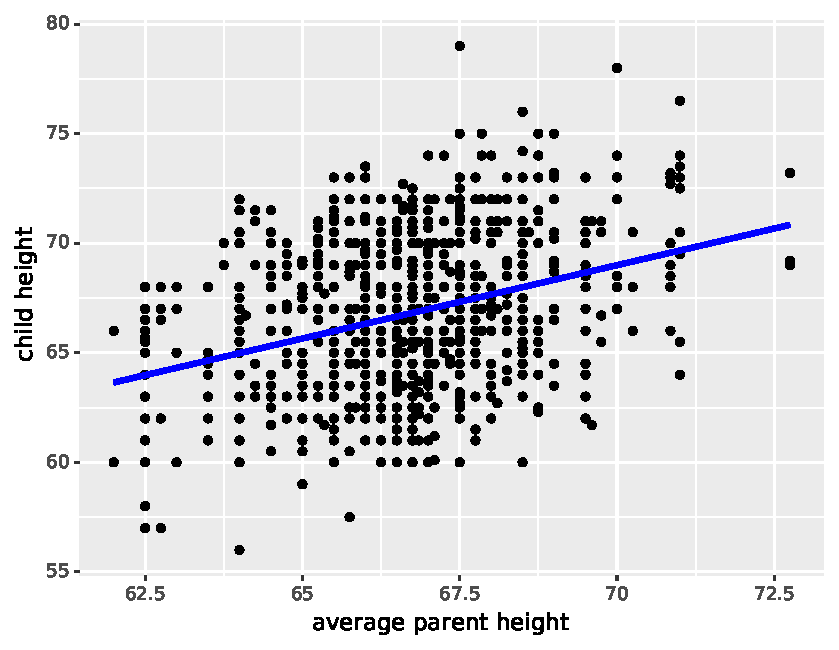
\includegraphics[width=0.9\textwidth]{../figures/galton_fit_sse.pdf}}
	\end{figure}
	
\end{frame}

\begin{frame}
	\frametitle{Strength of association between parent and child heights}
	
	Estimates of regression coefficient:
	
	\begin{equation}
	\text{child}_i = a + b * \text{parent}_i + \epsilon_i,
	\end{equation}
	
	\begin{itemize}
		\item Least squares / maximum likelihood: $b=0.67$
		\item Absolute deviance: $b=0.57$
		\item Fourth power: $b=0.73$
	\end{itemize}
	
\end{frame}

\begin{frame}
	\frametitle{Regression to mean}
	
	\begin{figure}[ht]
		\centerline{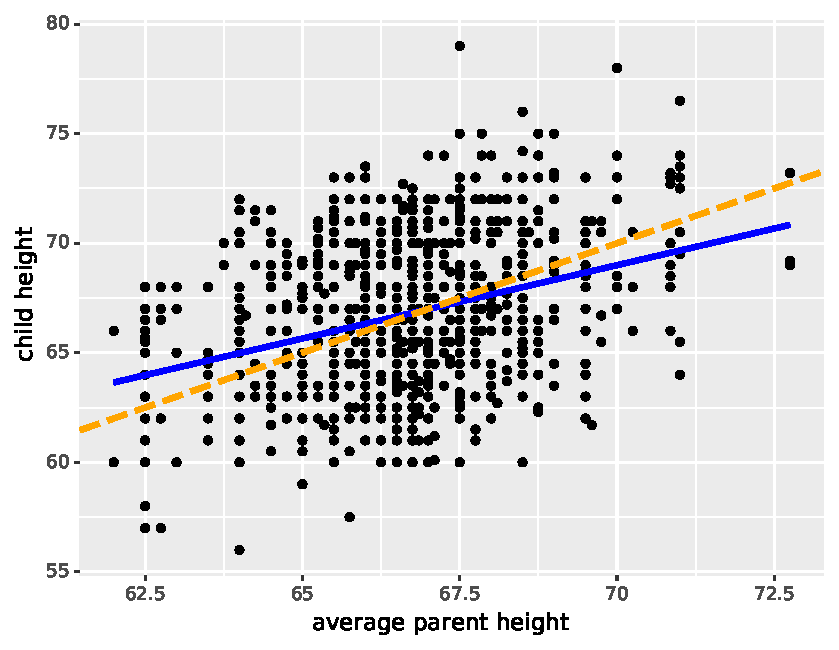
\includegraphics[width=0.9\textwidth]{../figures/galton_regression_to_mean.pdf}}
	\end{figure}
	
\end{frame}

\begin{frame}
	
	\Large Questions?
\end{frame}

\section{Model based thinking}
\frame{\tableofcontents[currentsection]}

\begin{frame}
	\frametitle{Regression is a model}
	
	\begin{equation}
	\text{child}_i = a + b * \text{parent}_i + \epsilon_i,
	\end{equation}
	
	and
	
	\begin{equation}
	\epsilon_i \sim \text{normal}(0, \sigma),
	\end{equation}
	
	is a model: an idealised version of reality.
	
\end{frame}

\begin{frame}
	\frametitle{Assumptions}
	
	Some of these:
	\begin{itemize}
		\item Linear association of average parental height with child height
		\item Variance of points around line is constant
		\item Normality of errors
		\item Male / female parent heights not separately important
		\item Sex of child unimportant in relationship
		\end{itemize}

\end{frame}

\begin{frame}
	\frametitle{Calculate errors: draw}
	
	\begin{figure}[ht]
		\centerline{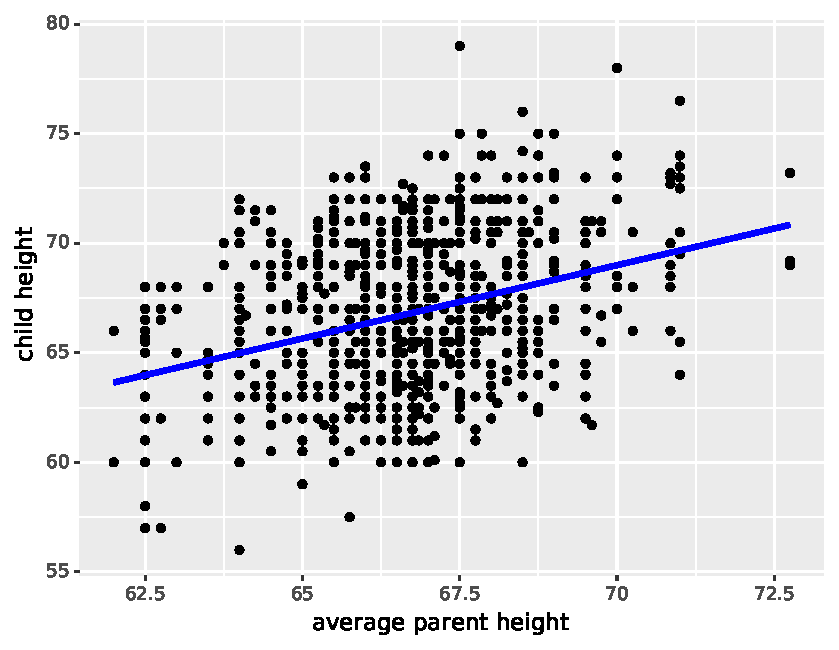
\includegraphics[width=0.9\textwidth]{../figures/galton_fit_sse.pdf}}
	\end{figure}
	
\end{frame}

\begin{frame}
	\frametitle{Checking linearity}
	
	\begin{figure}[ht]
		\centerline{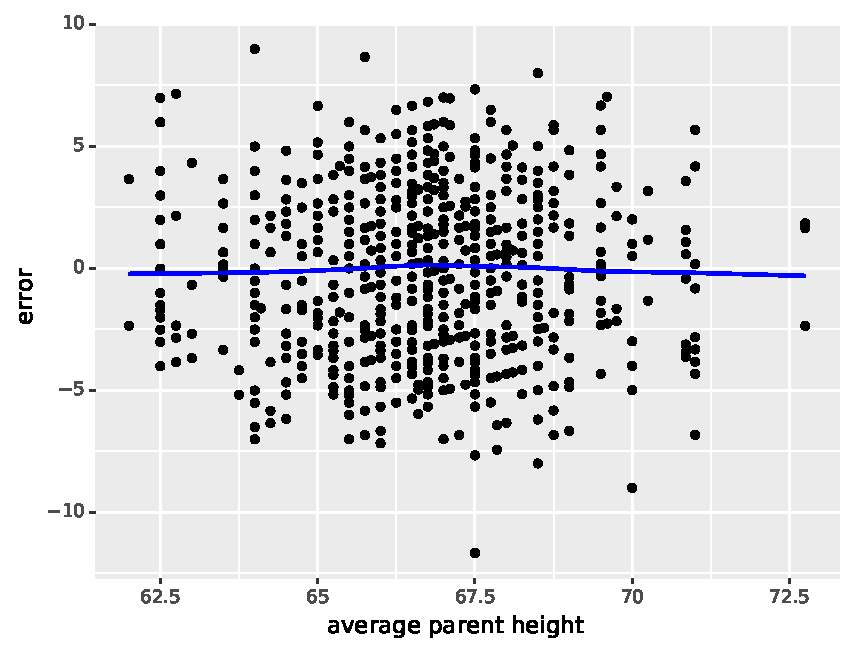
\includegraphics[width=0.9\textwidth]{../figures/galton_linearity.pdf}}
	\end{figure}
	
\end{frame}

\begin{frame}
	\frametitle{Checking variance homogeneity}
	
	\begin{figure}[ht]
		\centerline{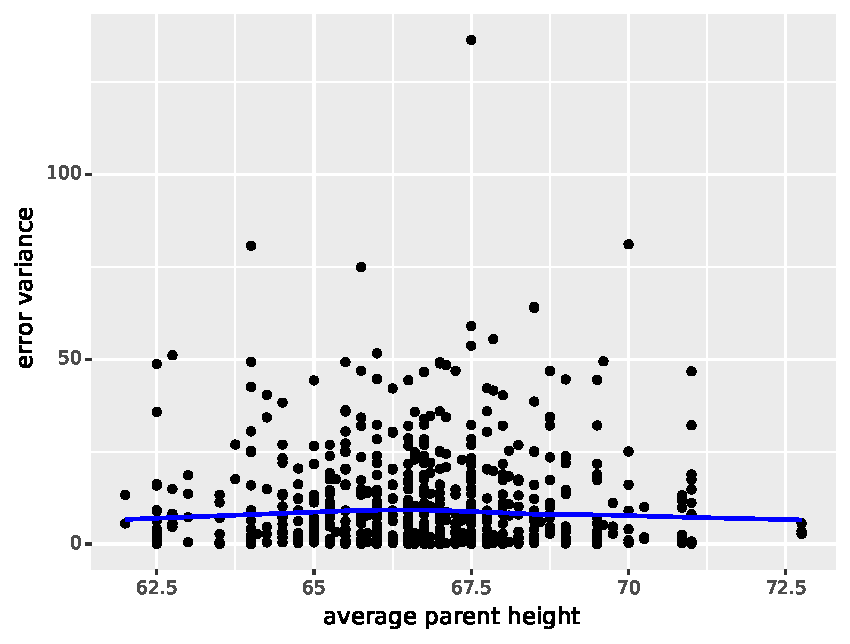
\includegraphics[width=0.9\textwidth]{../figures/galton_variance.pdf}}
	\end{figure}
	
\end{frame}

\begin{frame}
	
	\Large Questions?
\end{frame}

\section{Unpicking the signal from the noise}
\frame{\tableofcontents[currentsection]}

\begin{frame}
	\frametitle{How uncertain are we?}
	
	Least squares / maximum likelihood estimates:
	
	\begin{equation}
	\text{child}_i = 22.15 + 0.67 * \text{parent}_i + \epsilon_i,
	\end{equation}
	
	How representative are these of the population as a whole?
	
\end{frame}

\begin{frame}
	\frametitle{Gauging uncertainty: draw}
	
	Imagine:
	
	\begin{itemize}
		\item Repeatedly sampling from the population
		\item Each time calculating an estimate
	\end{itemize}
	
	$\implies$ variability in estimates dictates uncertainty.
	
\end{frame}

\begin{frame}
	\frametitle{Circularity}
	
	\begin{itemize}
		\item If we knew variability in estimates, we'd know how accurate they were
		\item But to do so, we need exact details of the population
	\end{itemize}
	
	How to resolve this ambiguity?
	
\end{frame}

\begin{frame}
	\frametitle{Two resolutions}
	
	\begin{itemize}
		\item Make mathematical assumptions about nature of population distribution. e.g. use CLT to determine normality
		\item Bootstrap sampling
	\end{itemize}
	
\end{frame}

\begin{frame}
	\frametitle{Bootstrap sampling}
	
	Since sample is drawn from the population, it should mirror it.
	
	\vspace{0.5cm}
	
	$\implies$ repeatedly draw new samples from our sample! And perform estimation on each.

	\vspace{0.5cm}
	
	Note sampling done with replacement.
	
\end{frame}


\begin{frame}
	\frametitle{Bootstrapped Galton samples}
	
	\begin{columns}
		\begin{column}{0.48\textwidth}
			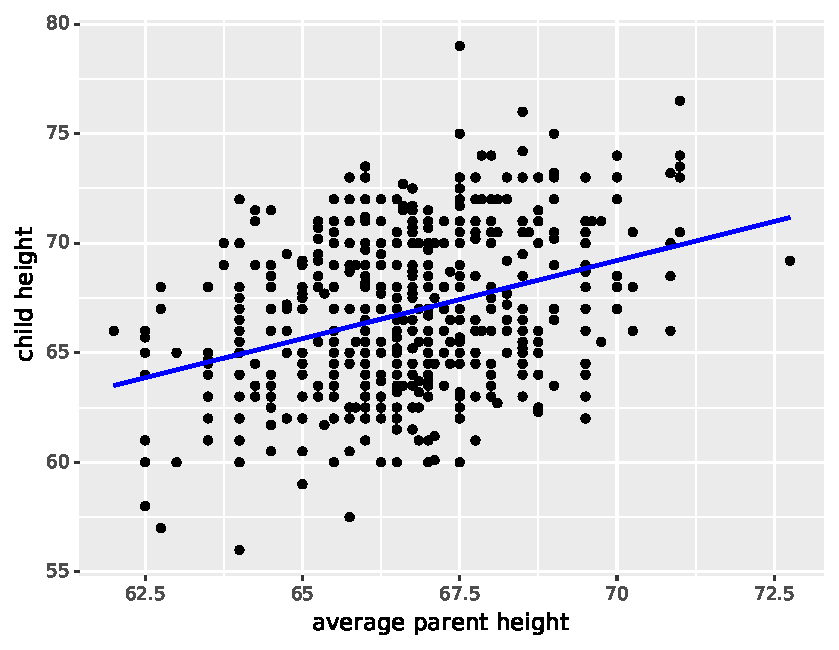
\includegraphics[width=0.9\textwidth]{../figures/galton_0.pdf}
			\end{column}
			\begin{column}{0.48\textwidth}
				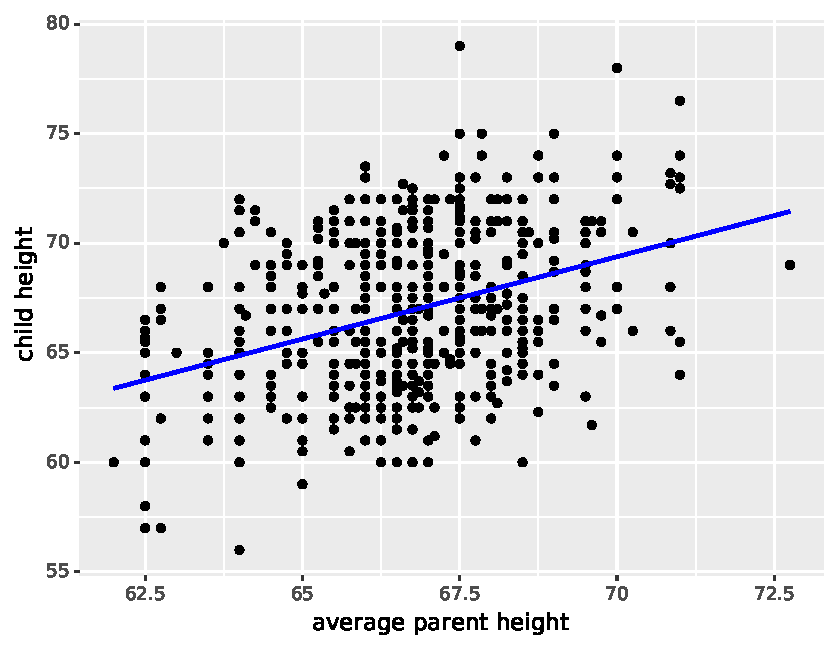
\includegraphics[width=0.9\textwidth]{../figures/galton_1.pdf}
			\end{column}
	\end{columns}
	
	\begin{columns}
		\begin{column}{0.48\textwidth}
			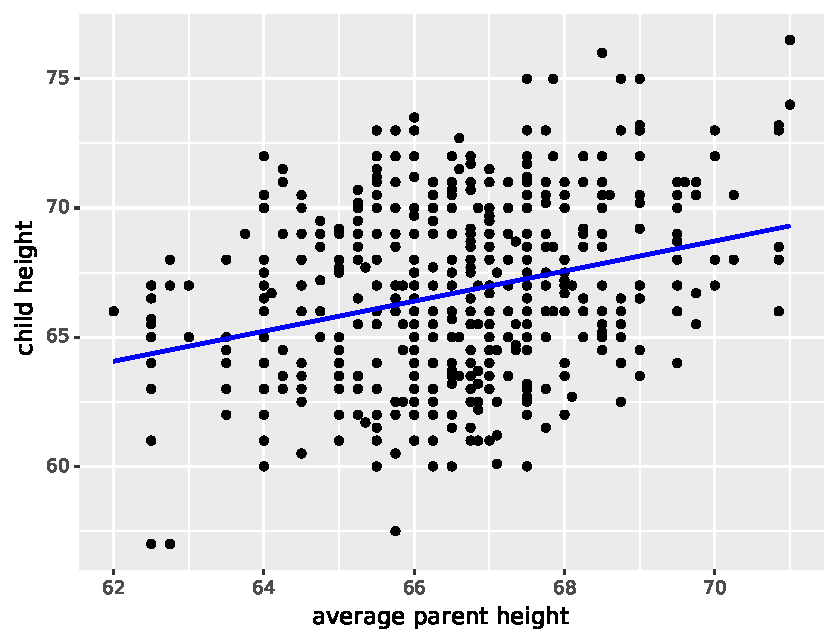
\includegraphics[width=0.9\textwidth]{../figures/galton_2.pdf}
		\end{column}
		\begin{column}{0.48\textwidth}
			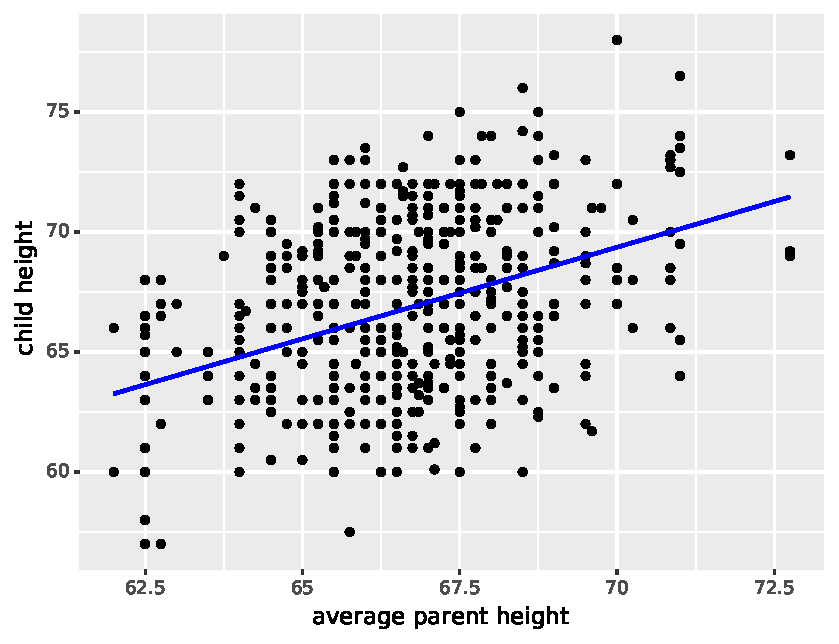
\includegraphics[width=0.9\textwidth]{../figures/galton_3.pdf}
		\end{column}
	\end{columns}
	
\end{frame}

\begin{frame}
	\frametitle{Bootstrapped Galton estimates: 4 bootstrapped samples}
	
	\begin{figure}[ht]
		\centerline{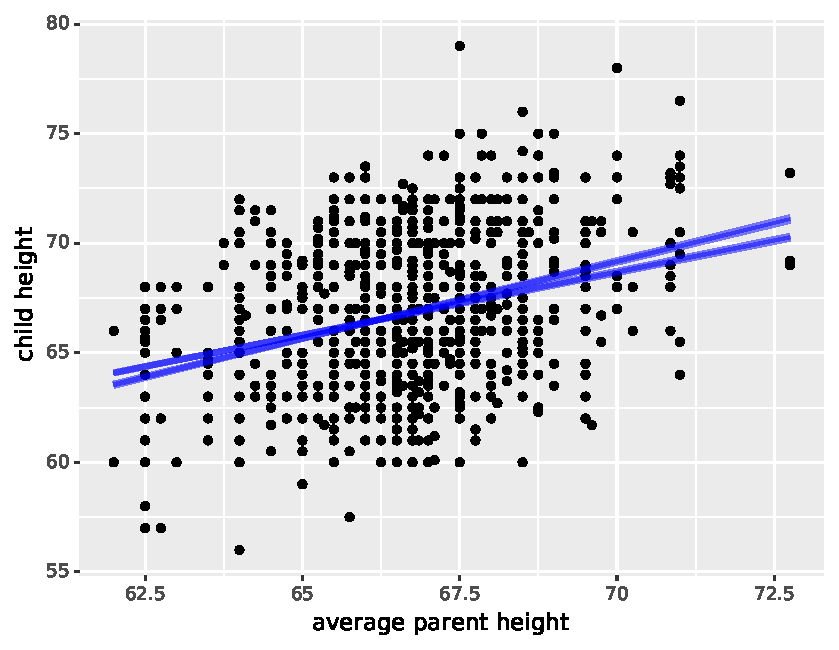
\includegraphics[width=0.9\textwidth]{../figures/galton_bootstrapped_estimates.pdf}}
	\end{figure}
	
\end{frame}

\begin{frame}
	\frametitle{Bootstrapped Galton estimates: 100 bootstrapped samples}
	
	\begin{figure}[ht]
		\centerline{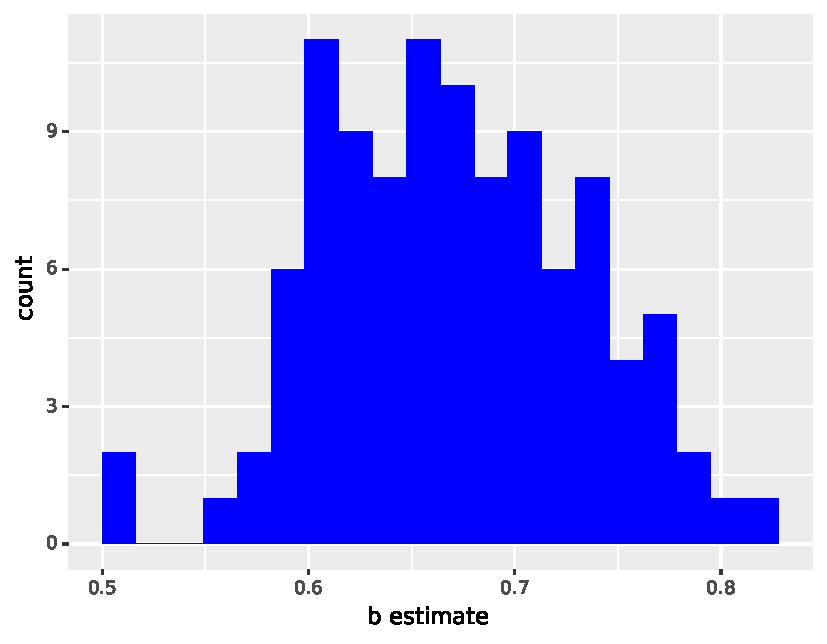
\includegraphics[width=0.9\textwidth]{../figures/galton_bootstrapped_estimates_histogram.pdf}}
	\end{figure}
	
\end{frame}

\begin{frame}
	\frametitle{When doesn't bootstrapping work?}
	
	\begin{itemize}
		\item Complex, highly structured data: for example, time series
		\item Large data $\implies$ too expensive
	\end{itemize}
	
	$\implies$ probability model based approach less cumbersome in these cases.
	
\end{frame}

\begin{frame}
	\frametitle{Conclusions}
	
	\begin{itemize}
		\item Data does not contain enough information about signals
		\item In statistics, we augment data with assumptions (embodied in randomness) $\implies$ separate signal from noise
		\item Simple associations are non-causal but shouldn't dampen our ambition
		\item Linear regression allows for quantification of relationships between two variables
		\item Linear regression, like all statistical assumptions, is a model which can be fallible
		\item Uncertainty in estimates can be obtained by bootstrap sampling
	\end{itemize}
	
\end{frame}

\begin{frame}
	\frametitle{That's it!}
	
	\Large Questions?
\end{frame}

\begin{frame}
	\frametitle{Further material}
	
	\begin{columns}
		\begin{column}{0.3\textwidth}
			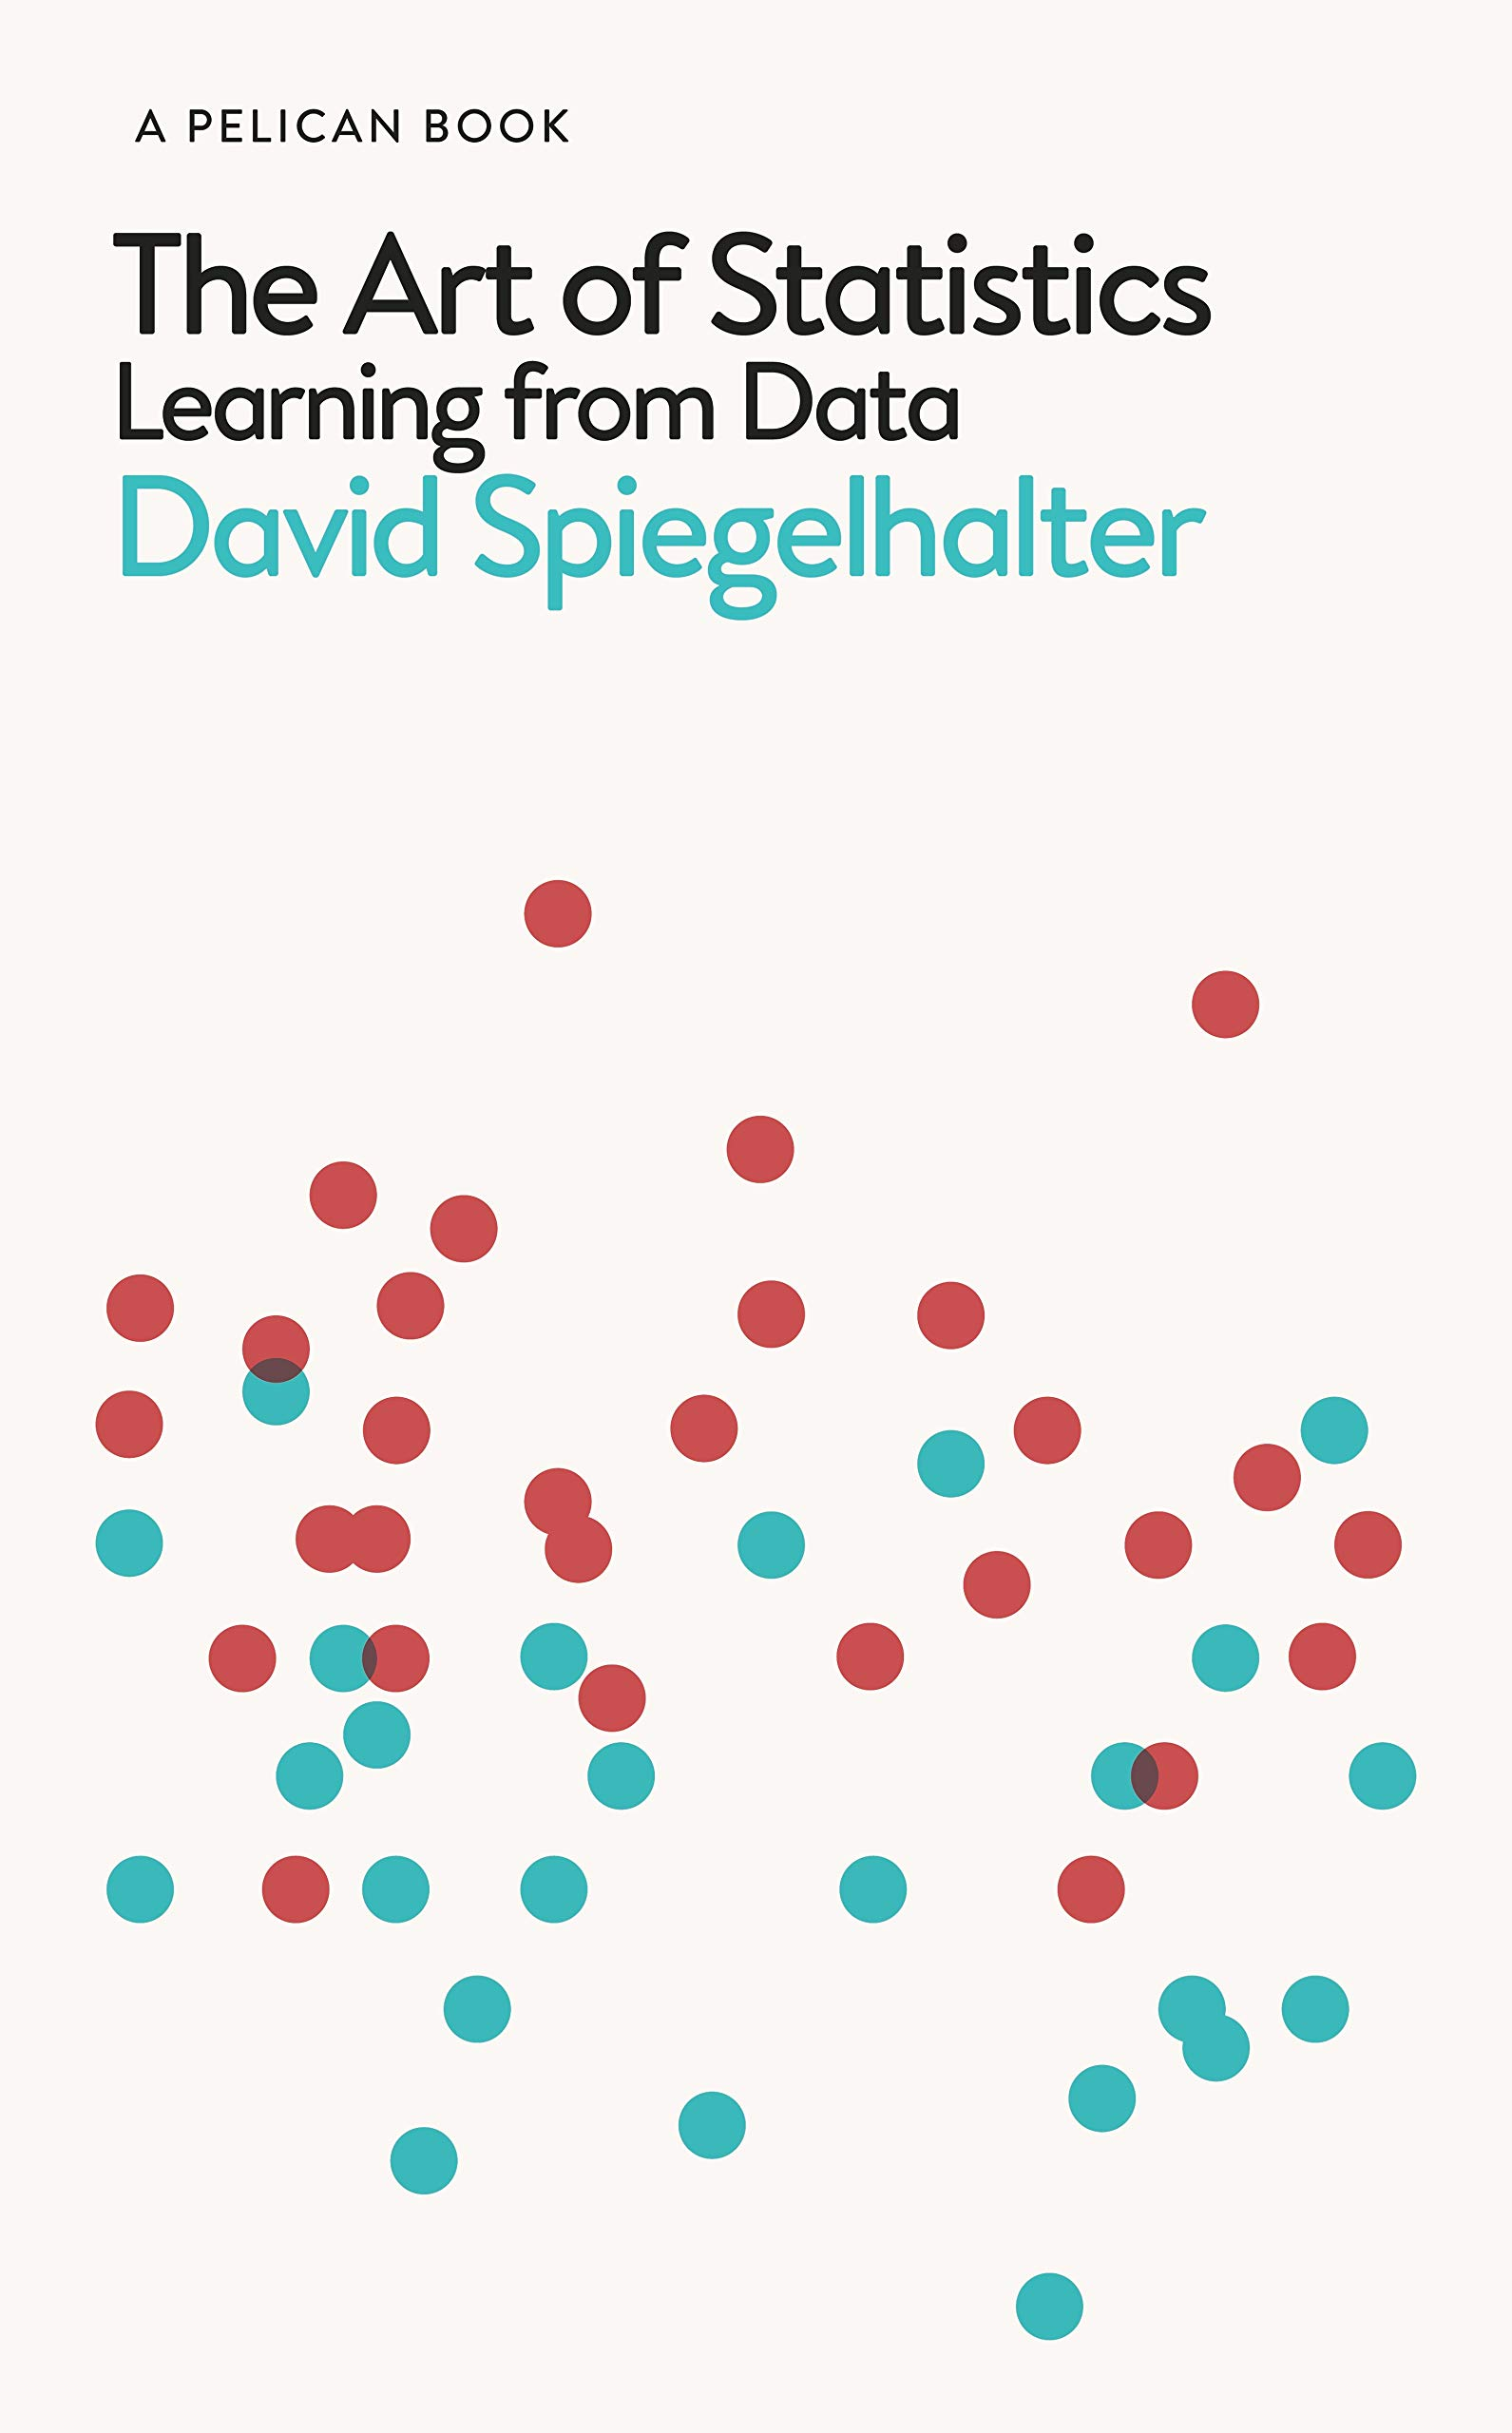
\includegraphics[width=0.9\textwidth]{../figures/art_of_statistics.jpeg}
		\end{column}
		\begin{column}{0.3\textwidth}
			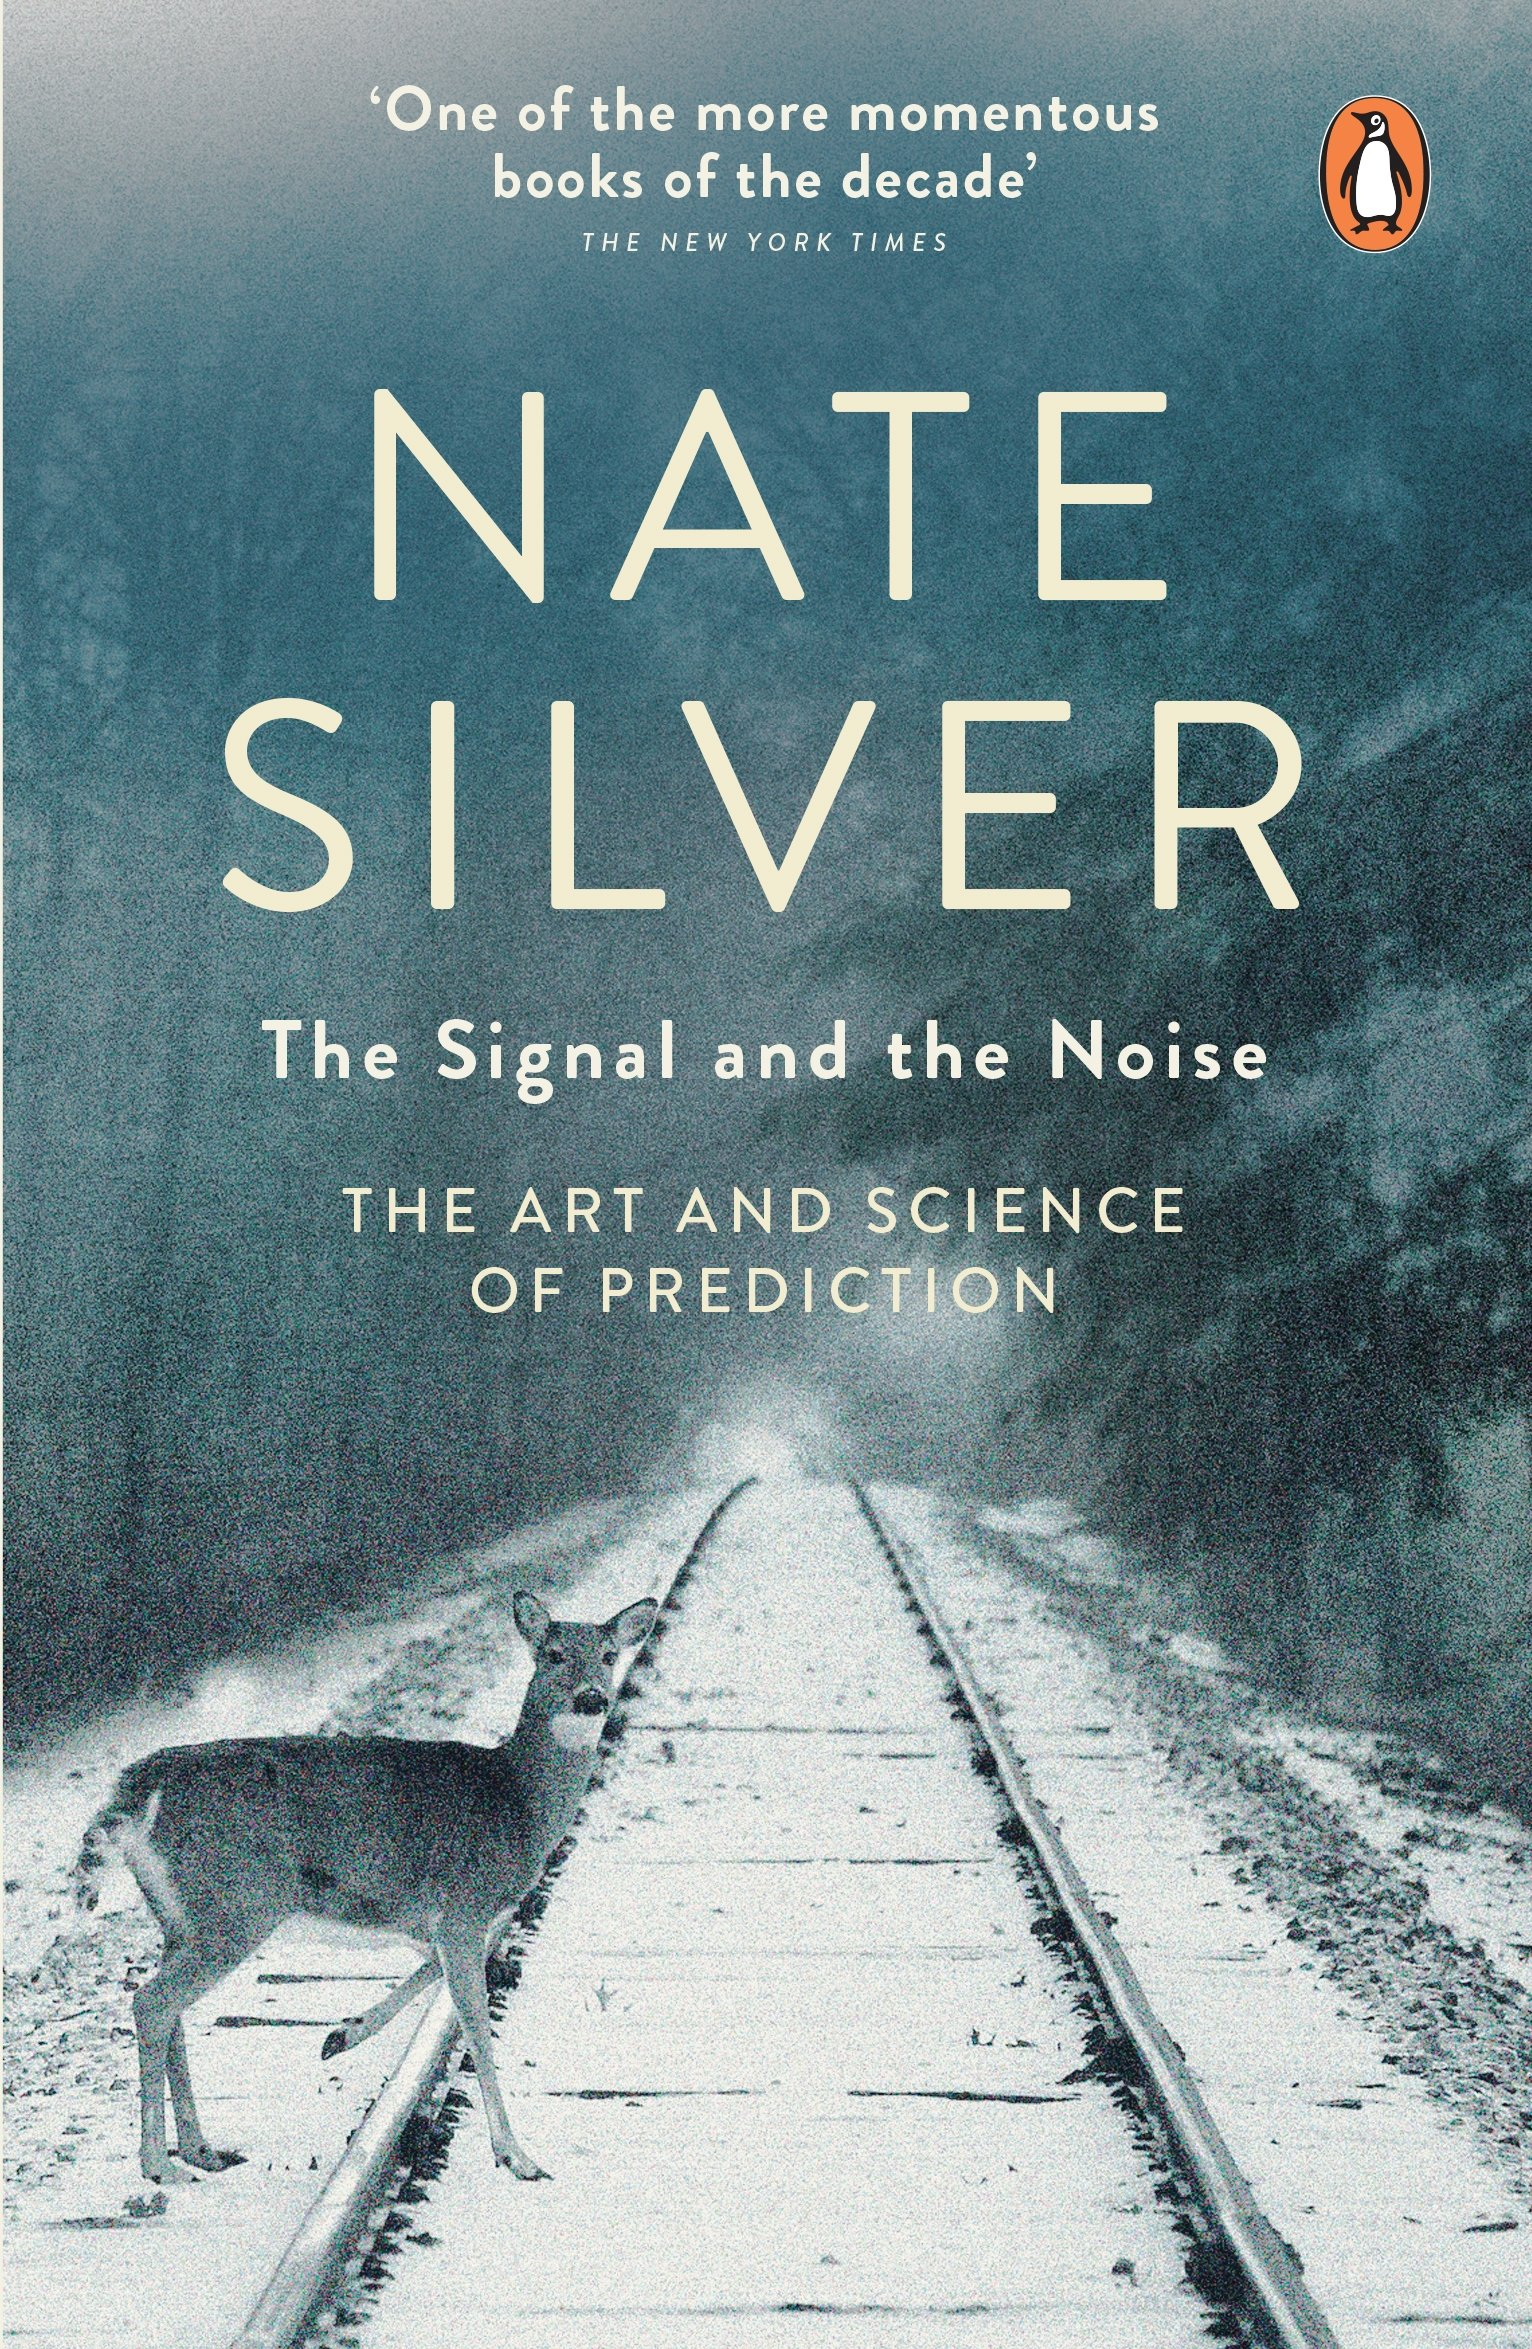
\includegraphics[width=0.9\textwidth]{../figures/signal_noise.jpeg}
		\end{column}
		\begin{column}{0.3\textwidth}
			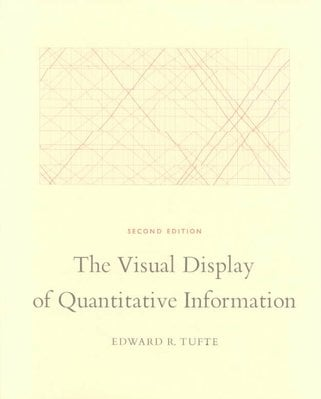
\includegraphics[width=0.9\textwidth]{../figures/tufte.jpeg}
		\end{column}
	\end{columns}
	
\end{frame}


\end{document}
